%!TEX root = ../main.tex



\section{Εισαγωγή}

Ο χρήστης της πλατφόρμας είναι ένας μηχανικός/data scientist ο οποίος δουλεύει σε μια εταιρία που αναπτύσσει μία πλατφόρμα Forex Trading. Αυτός ο μηχανικός δουλεύει πάνω σε ένα Σύστημα Συστάσεων (RS). Ο μηχανικός αυτός έχει στη διάθεση του ένα μεγάλο αριθμό από δεδομένα των συναλλαγών των πελατών τα οποία θέλει να αξιοποιήσει στο RS που υλοποιεί. Με άλλα λόγια έχει στη διάθεση του ένα σύνολο από έμμεσες αξιολογήσεις, από τις οποίες θα χρειαστεί να εξάγει κάποιες «ψευδο-αξιολογήσεις» με τις οποίες θα εκπαιδευτεί το RS.

Όπως αναφέραμε και προηγουμένως η εξαγωγή των ψευδο-αξιολογήσεων μπορεί να χωριστεί σε τρία στάδια:

\begin{enumerate}
	\item Ανάλυση και δημιουργία «διαισθήσεων» πάνω στα δεδομένα
	\item Επιλογή των χαρακτηριστικών των δεδομένων για τον υπολογισμό των ψευδο-αξιολογήσεων και αξιολόγηση των ψευδο-αξιολογήσεων
	\item Αξιολόγηση των αποτελεσμάτων του Συστήματος Συστάσεων \ldots
\end{enumerate} 	

Έτσι και το Visfx χωρίζεται αντίστοιχα σε τρεις ενότητες, στην Data Overview, Feature Selection, και Recommendations.

\section{Επισκόπηση Δεδομένων – Data Overview}

Ξεκινώντας στην καρτέλα Data Overview ο μηχανικός μπορεί να διαλέξει την χρονική περίοδο πάνω στην οποία θέλει να δουλέψει. Αρχικά χαιρετίζεται με ένα Parallel Coordinates διάγραμμα μέσω του οποίου μπορεί γρήγορα και αποτελεσματικά να δει το σύνολο των δεδομένων του και να κάνει οπτικοποιημένες αναζητήσεις πάνω σ’ αυτά. Ο χρήστης μπορεί να είτε να φιλτράρει τους άξονες μαρκάροντας περιοχές πάνω σ’ αυτούς, είτε να χρησιμοποιήσει τα πεδία αμέσως κάτω από το διάγραμμα. Κάθε γραμμή στο διάγραμμα αναπαριστά μία συναλλαγή, ενώ οι γραμμές με το ίδιο χρώμα είναι συναλλαγές από την ίδια χώρα. Για παράδειγμα ξεκινώντας από τα αριστερά βλέπουμε ότι ο Provider με ID 911888 που είναι από την Σιγκαπούρη άνοιξε μία συναλλαγή XAU/USD την τάδε ημερομηνία, έκλεισε την δείνα με μικρό Amount και το Net PnL ήταν μικρό αλλά αρνητικό.

\begin{figure}[H]
  \centering
  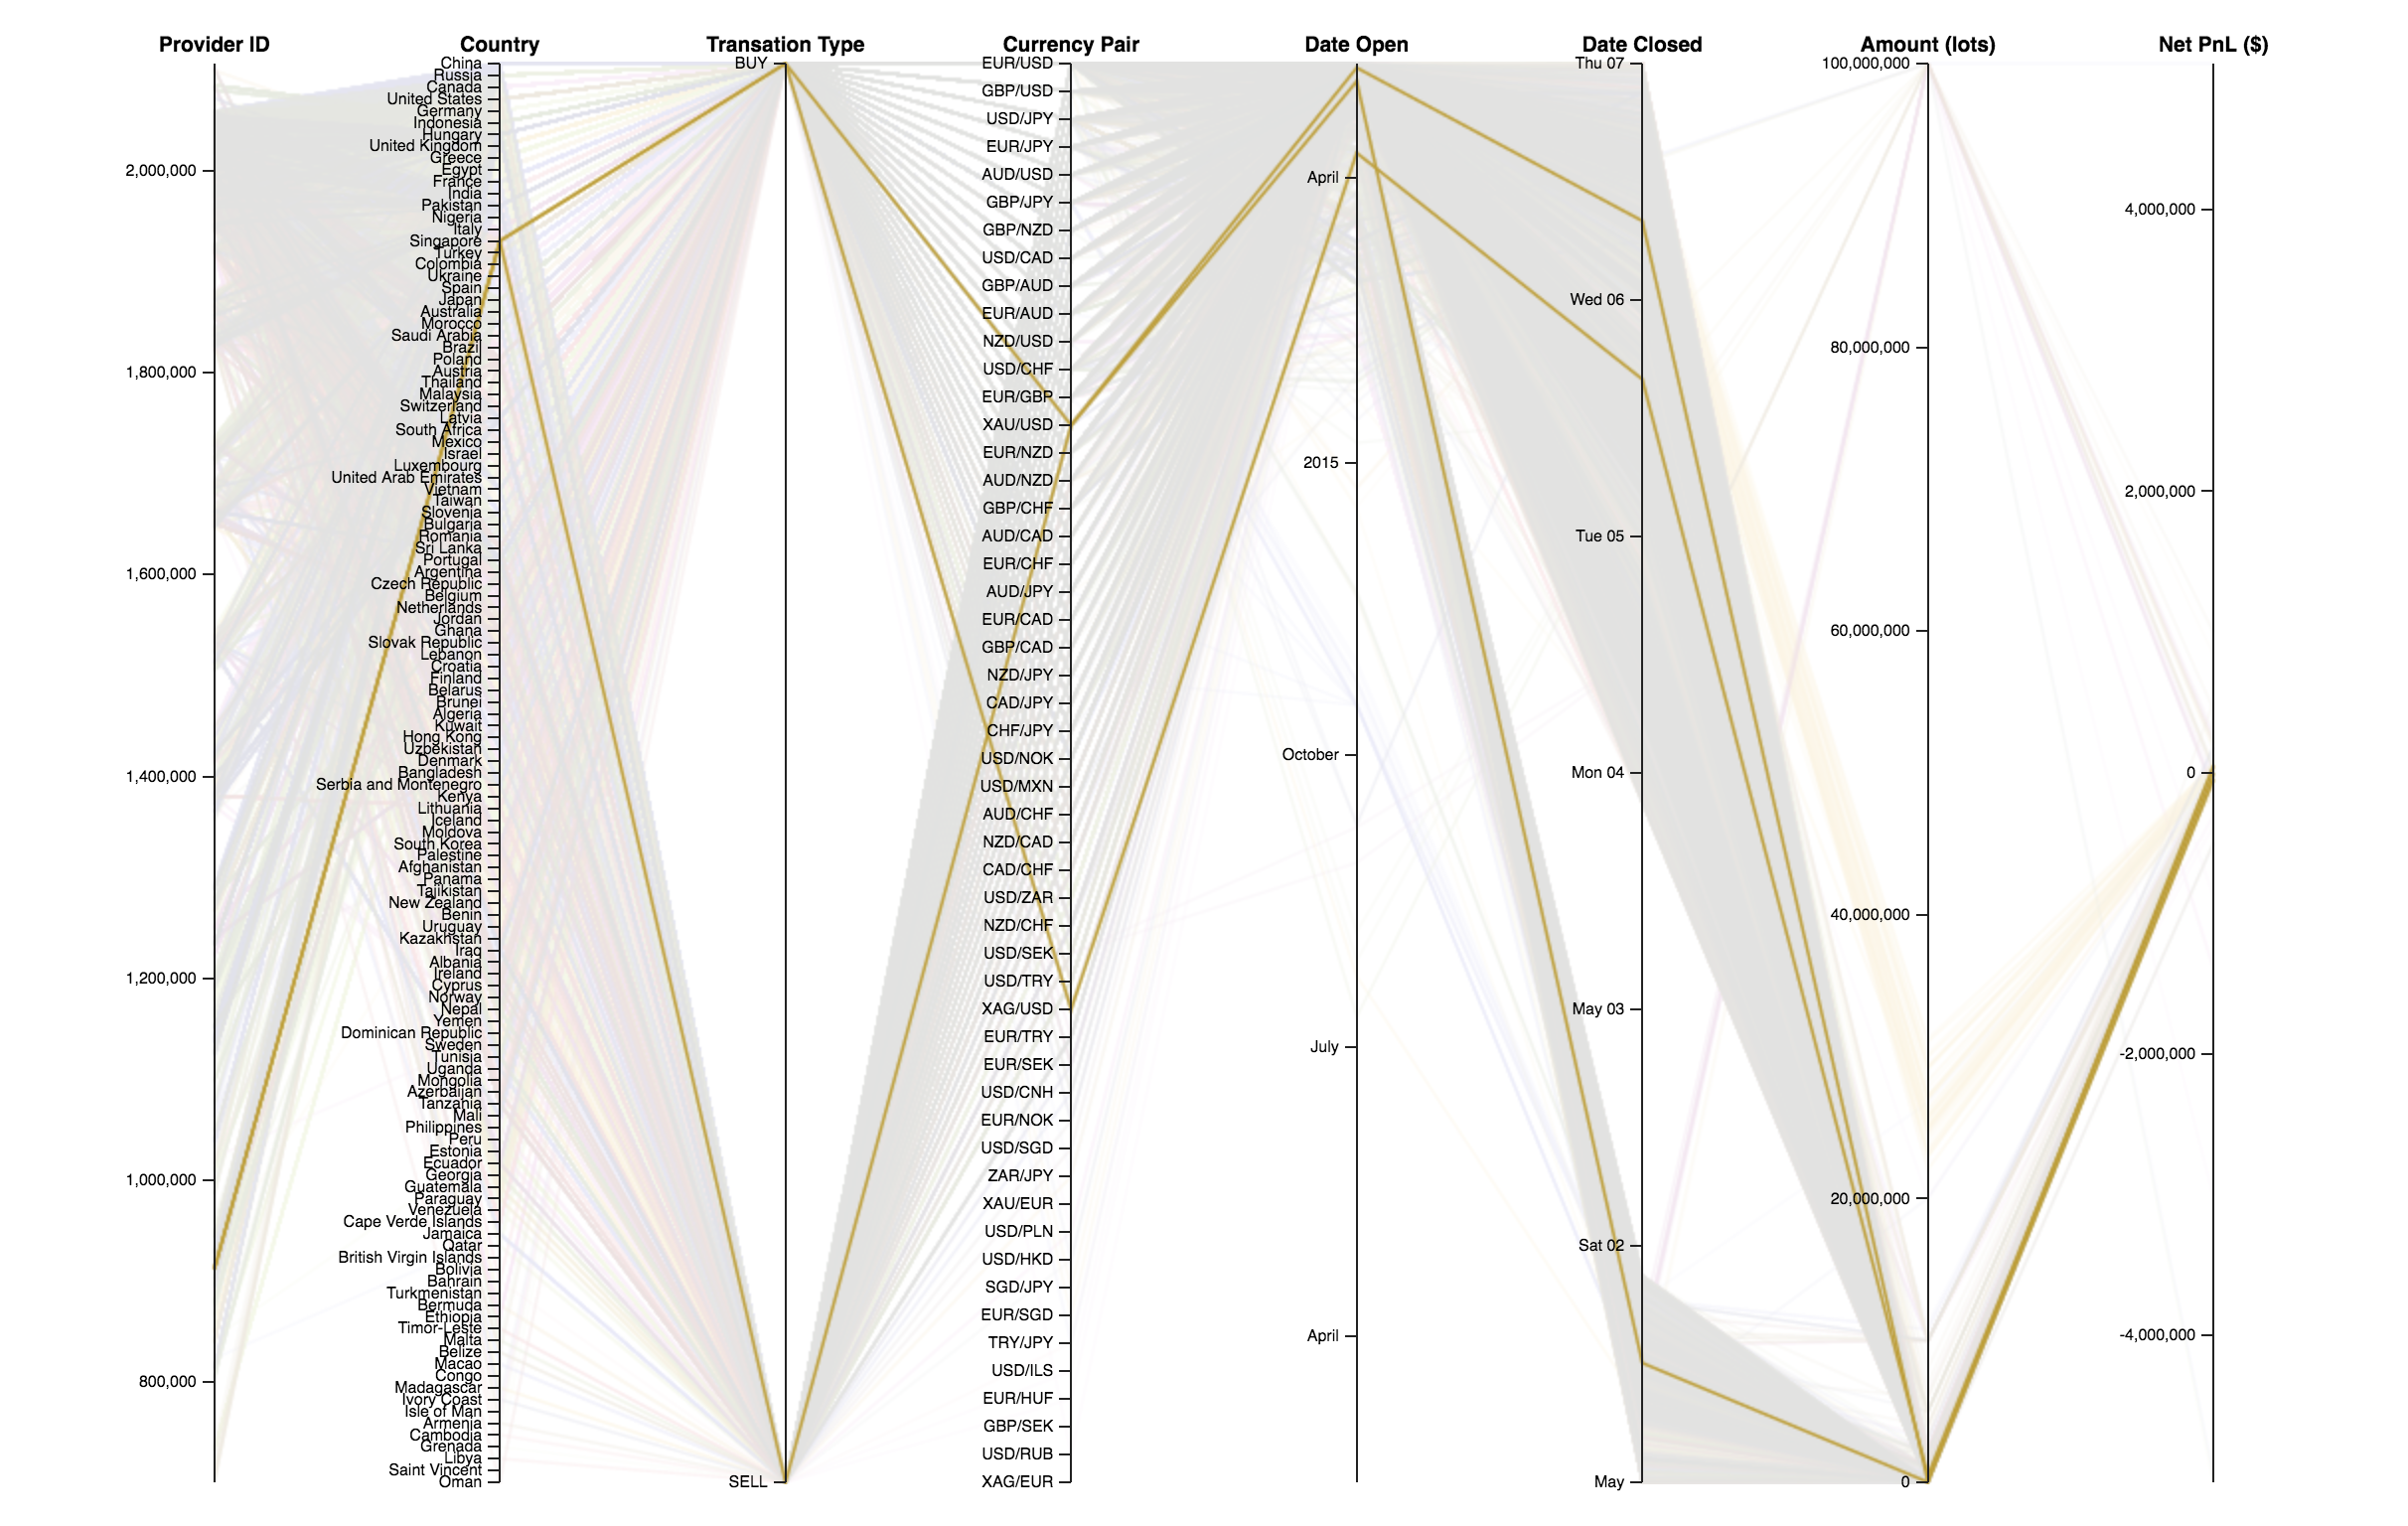
\includegraphics[width=\textwidth]{parcoords_single}
  \label{fig:parcoords_single}
\end{figure}

Επίσης ο χρήστης μπορεί να κάνει πιο περίπλοκες αναζητήσεις. Για παράδειγμα μπορεί να επιλέξει πάνω στους άξονες τις συναλλαγές που έγιναν από τις Ηνωμένες Πολιτείες της Αμερικής στο ζεύγος GBP/USD και USD/CAD και άνοιξαν μέσα στον Απρίλιο:

\begin{figure}[H]
  \centering
  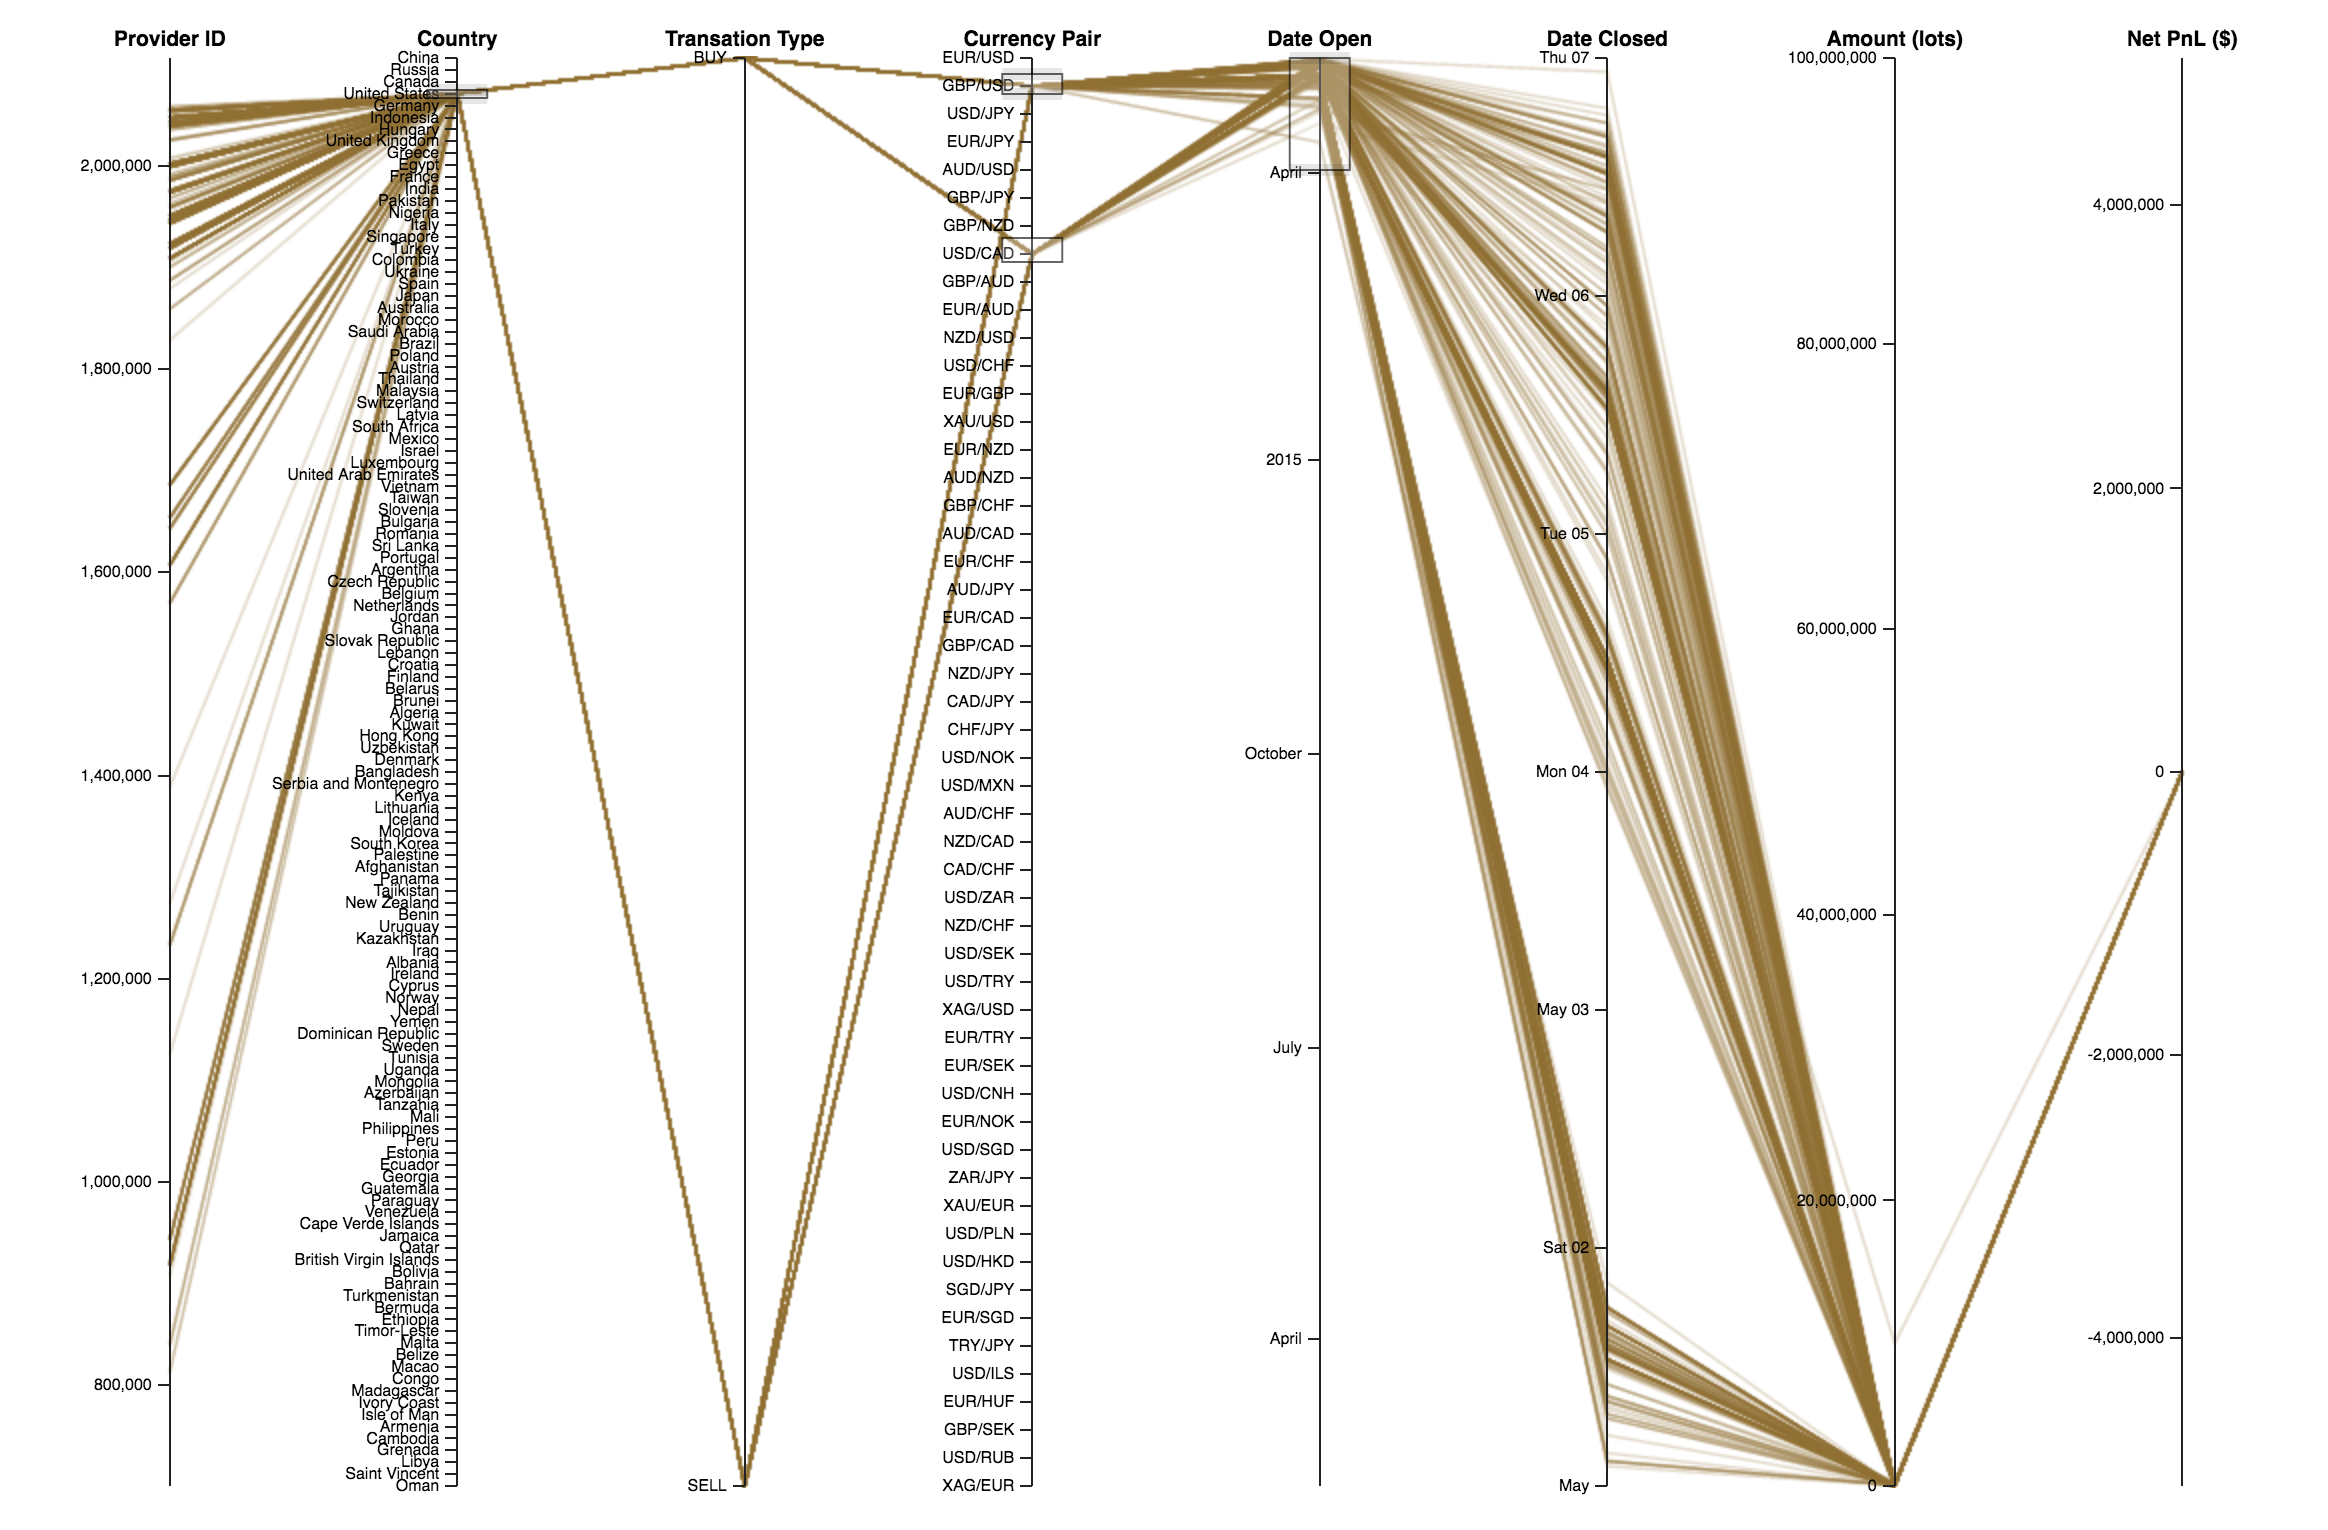
\includegraphics[width=\textwidth]{parcoords_complex}
  \label{fig:parcoords_complex}
\end{figure}

Κάνοντας αυτή την αναζήτηση μπορεί να δει πως συμπεριφέρονται οι χρηματιστές σε μία χώρα όταν συναλλάσσονται ένα συγκεκριμένο ζεύγος και ρυθμίζονται το παράθυρο του Date Open να δει πως η διάρκεια της συναλλαγής επηρεάζει τα κέρδη της.

Επεκτείνοντας περισσότερο, αν δούμε τις συναλλαγές για το ζεύγος EUR/USD βλέπουμε ότι αυτές που είχαν μικρότερη διάρκεια ήταν αρκετά πιο κερδοφόρες απ’ αυτές με διάρκεια πάνω από εβδομάδα. Γι’ αυτό επιλέξαμε στη συνέχεια σαν χαρακτηριστικό την διάρκεια των συναλλαγών (Trade Duration)

\begin{figure}[H]
  \centering
  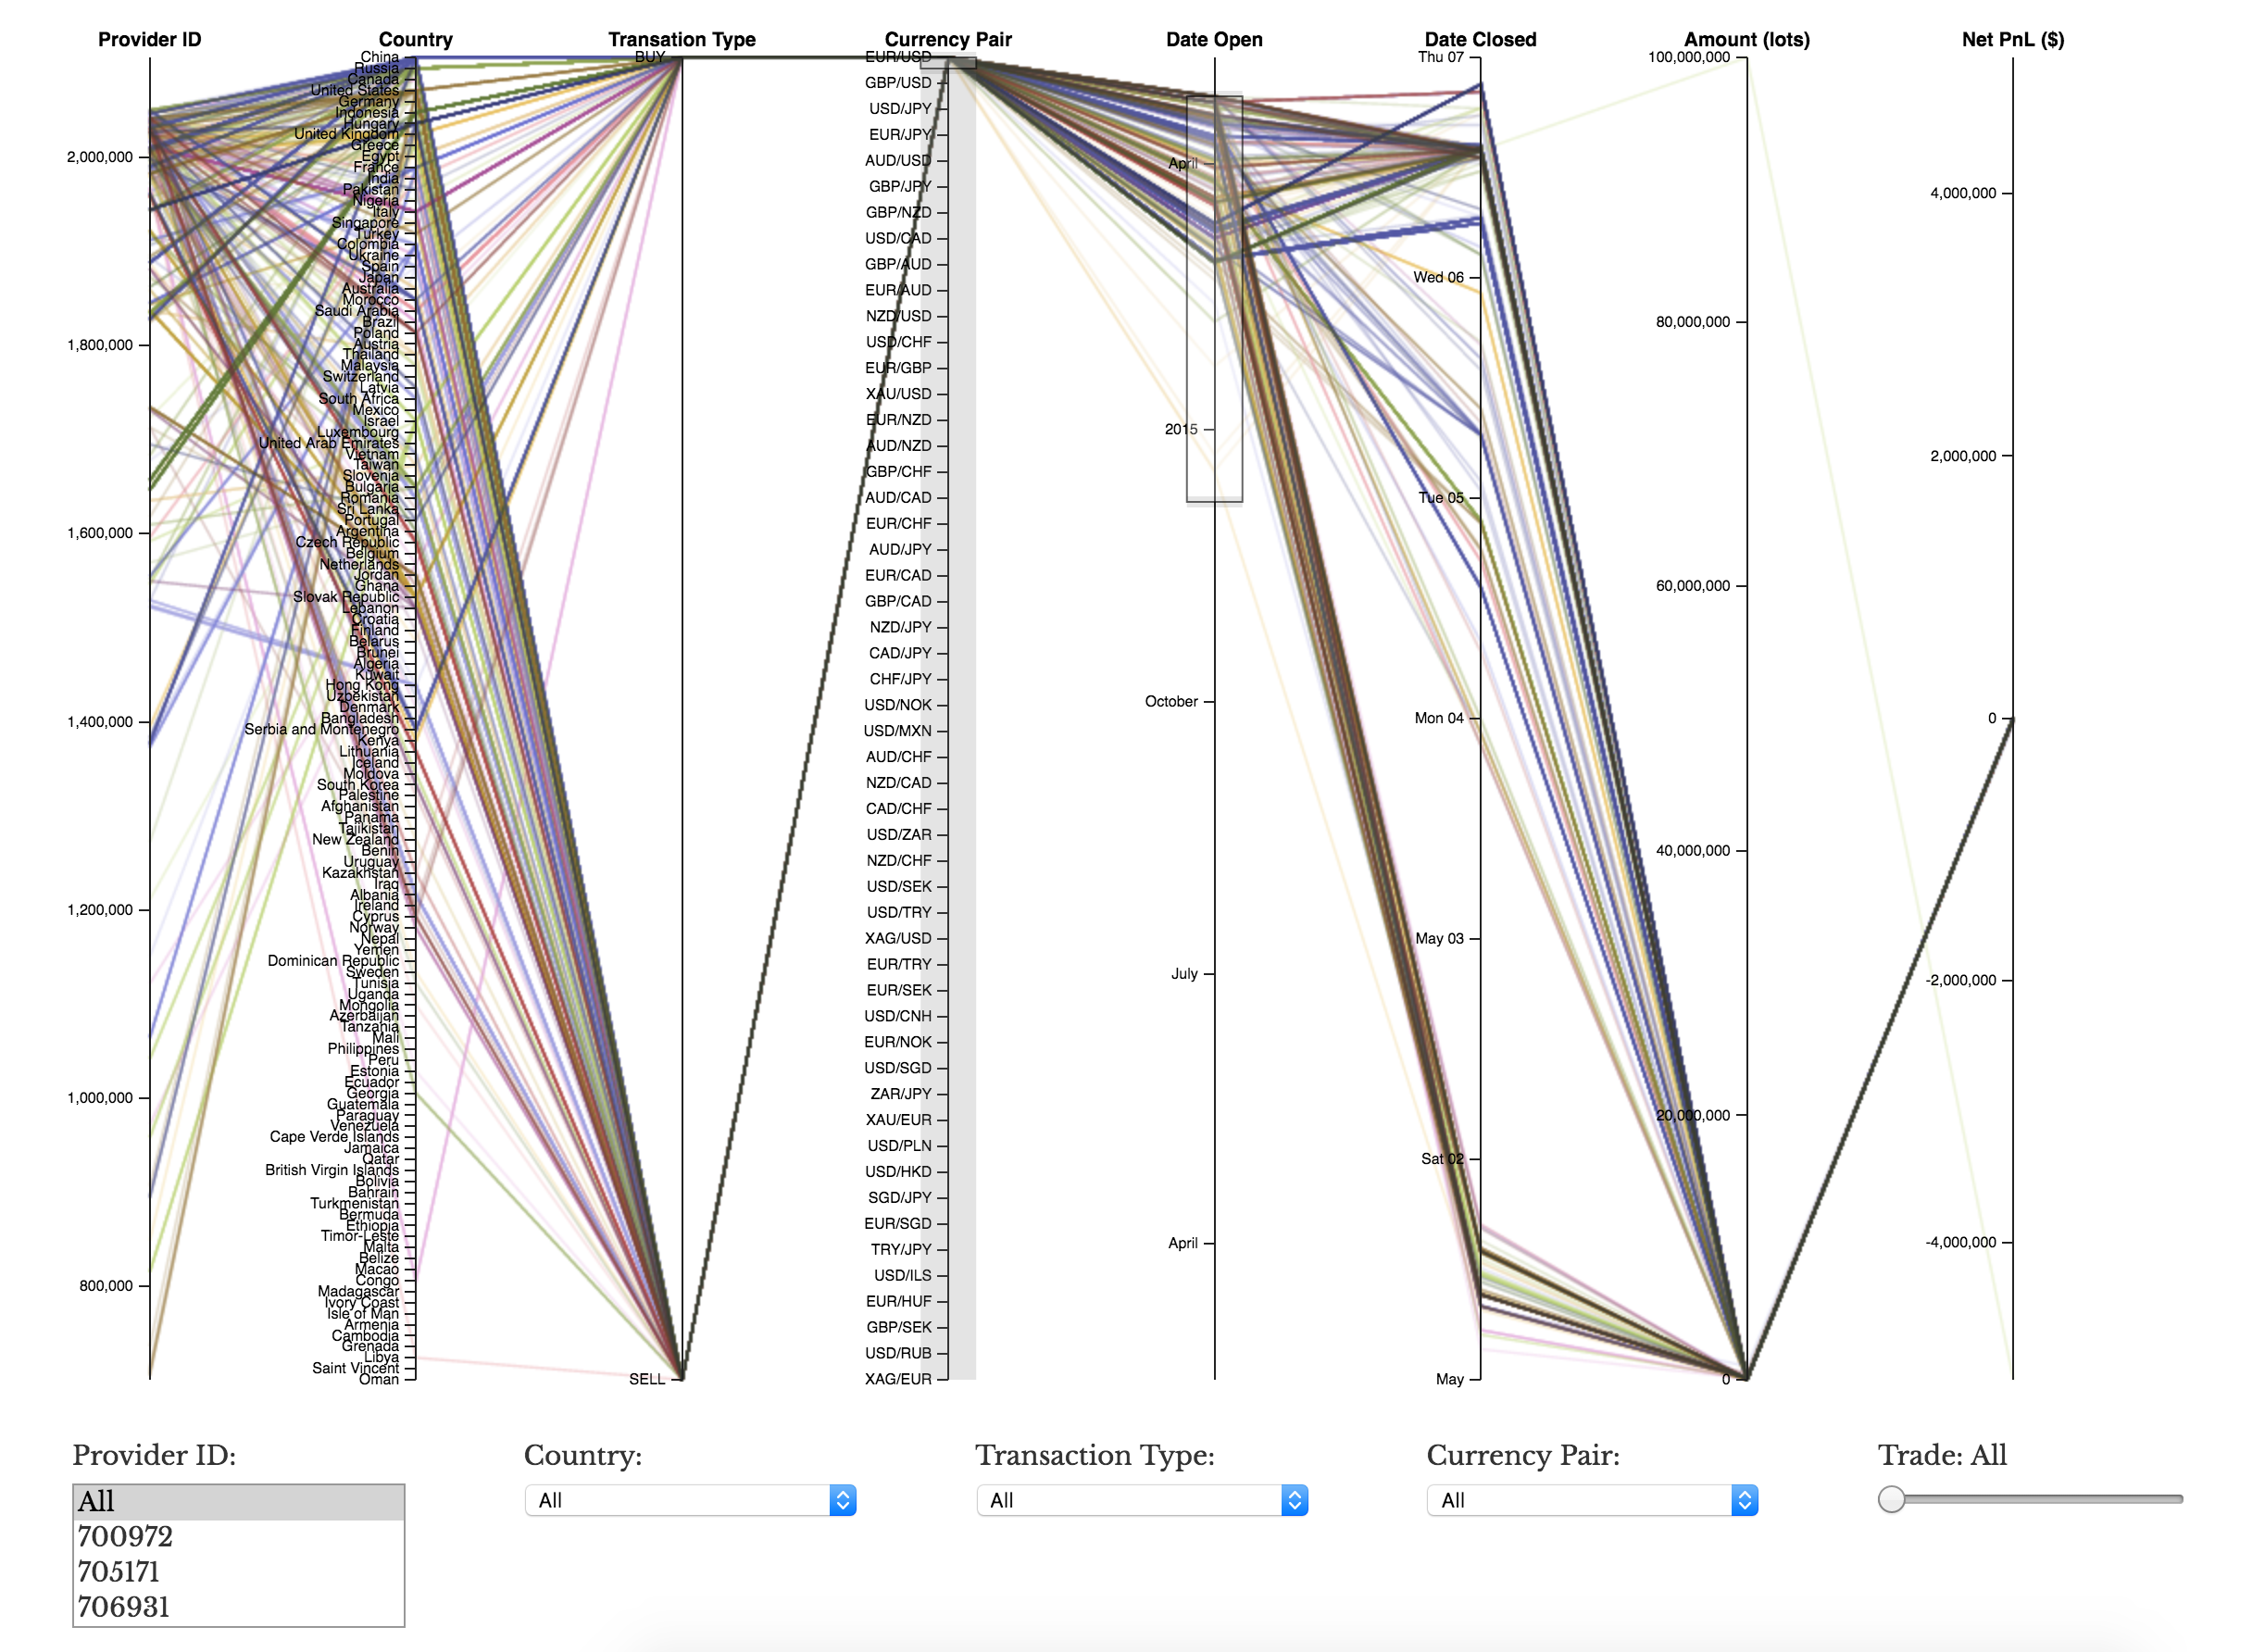
\includegraphics[width=\textwidth]{parcoords_late}
  \label{fig:parcoords_late}
\end{figure}
\hfill
\begin{figure}[H]
  \centering
  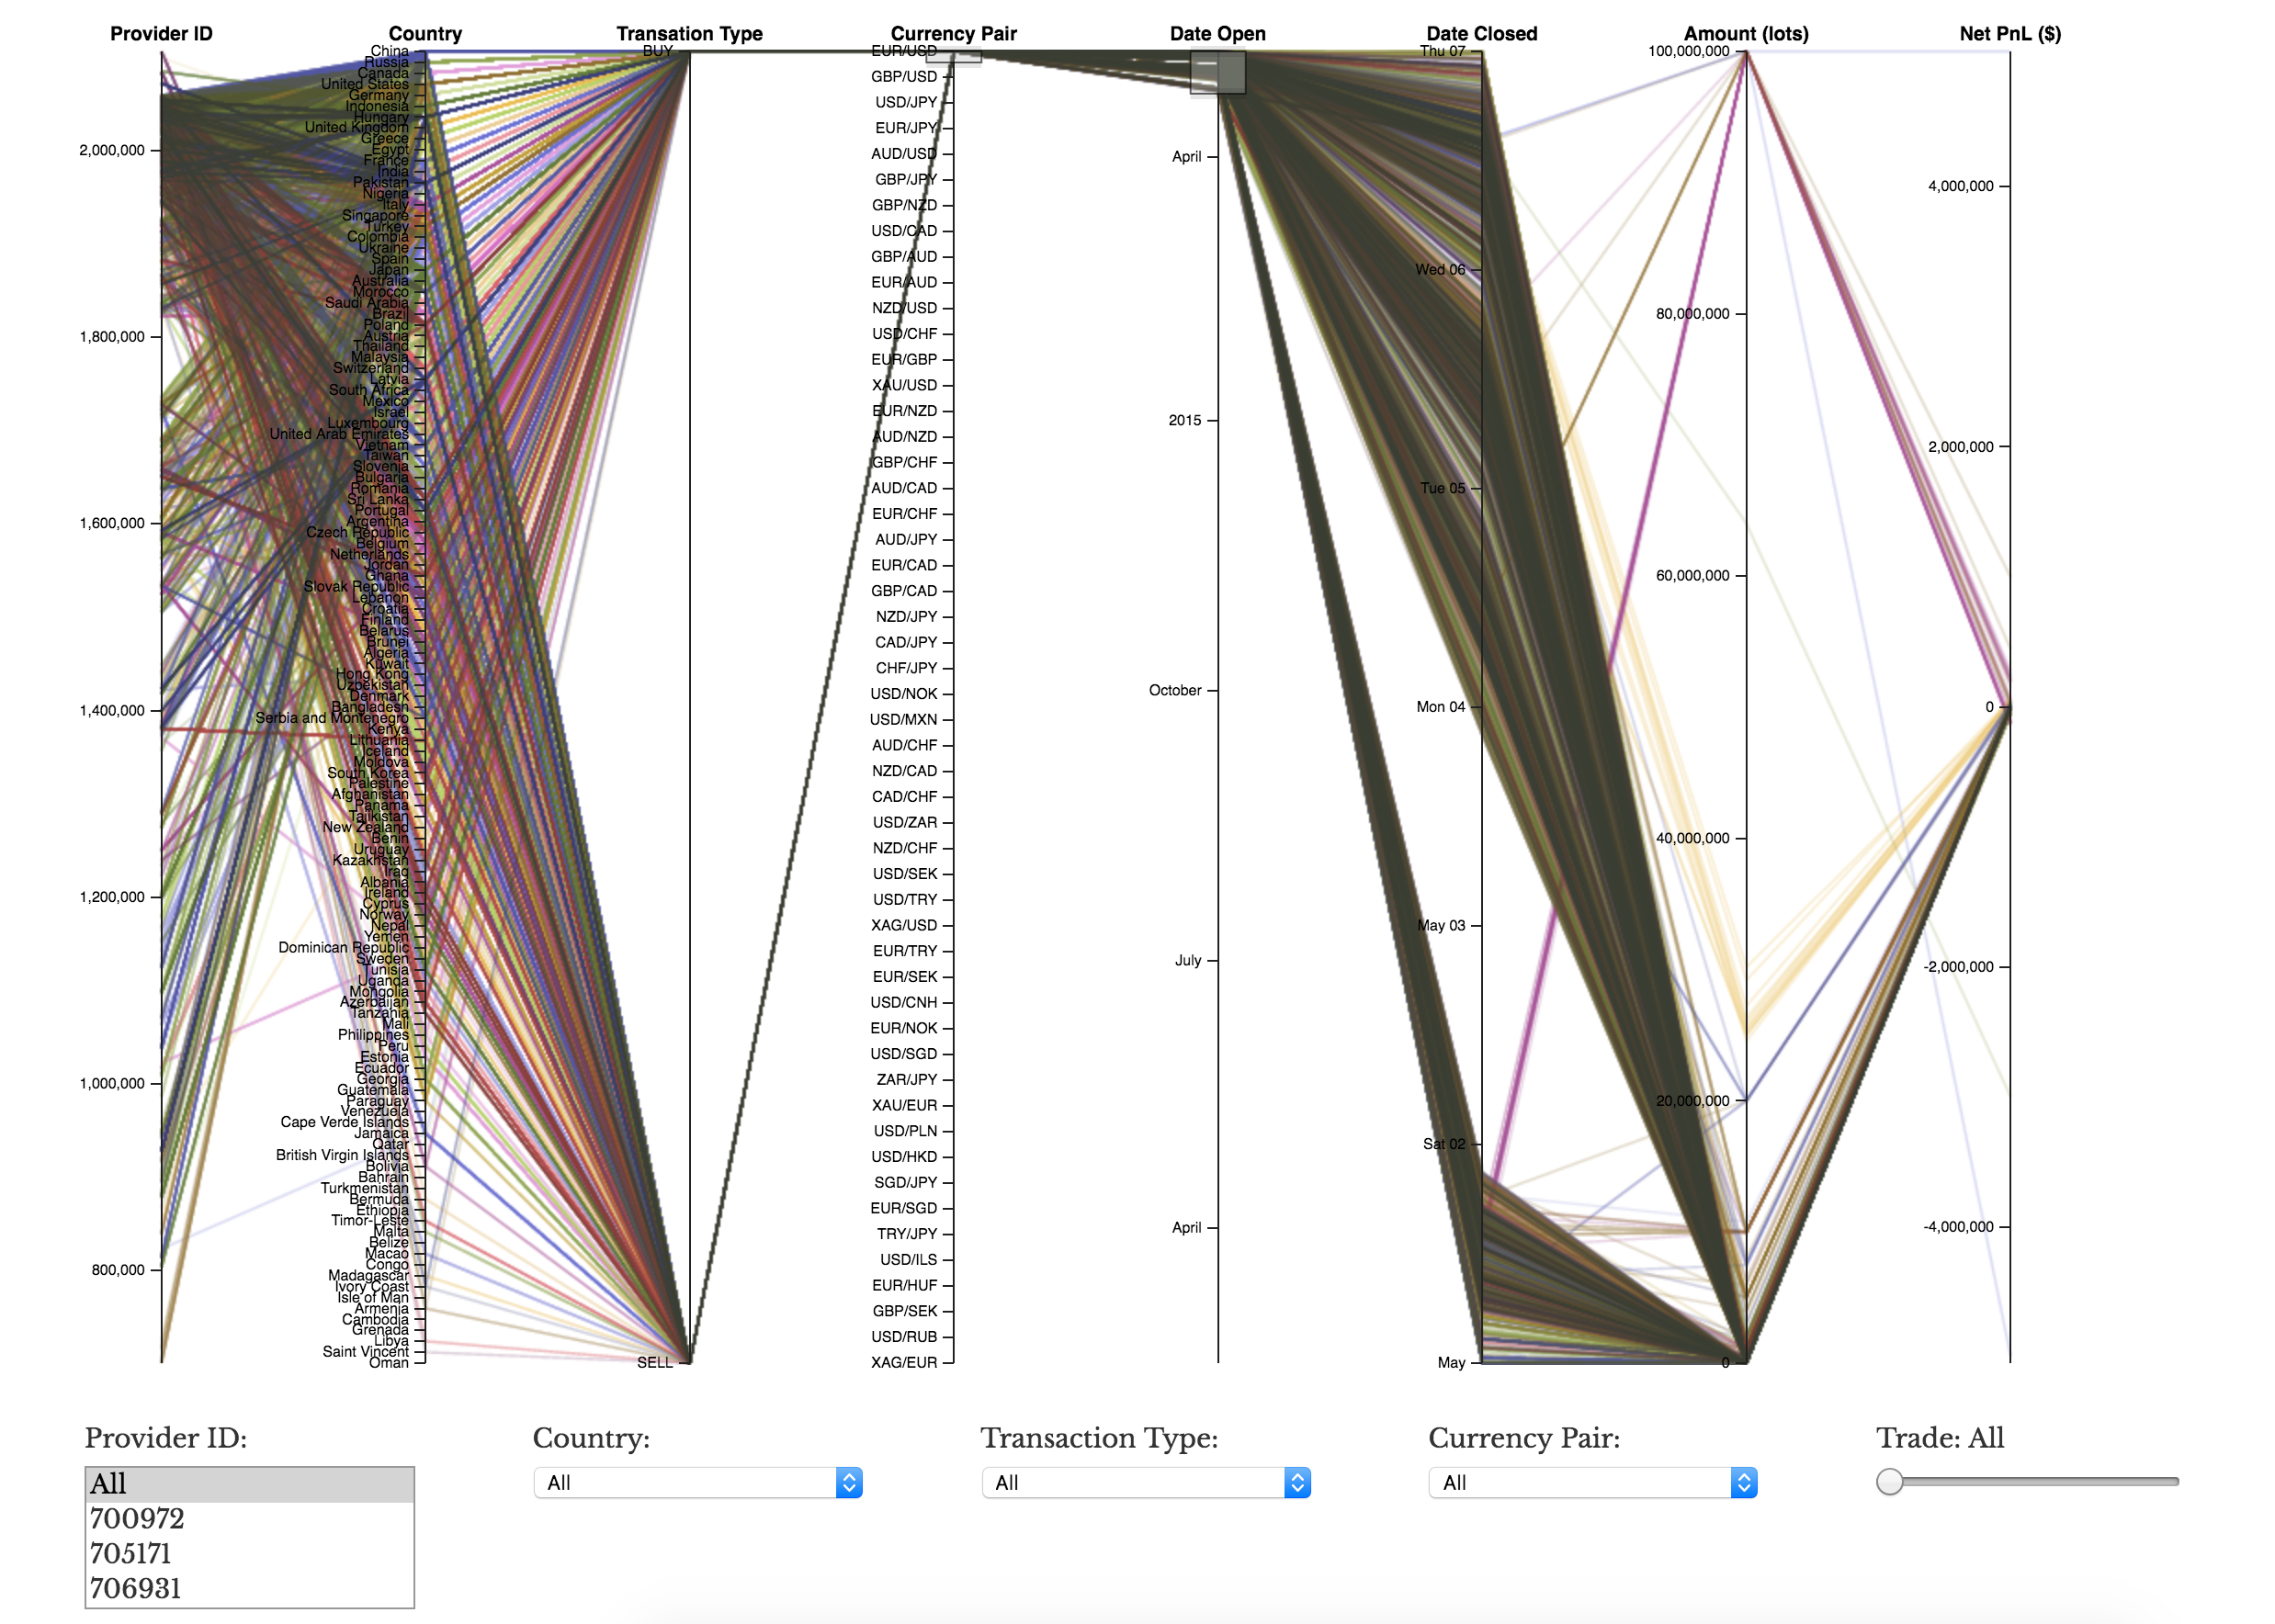
\includegraphics[width=\textwidth]{parcoords_early}
  \label{fig:parcoords_early}
\end{figure}

Στη συνέχεια ο χρήστης μπορεί δει πιο αναλυτικά πτυχές των δεδομένων μέσω των επόμενων γραφημάτων.

\begin{figure}[H]
  \centering
  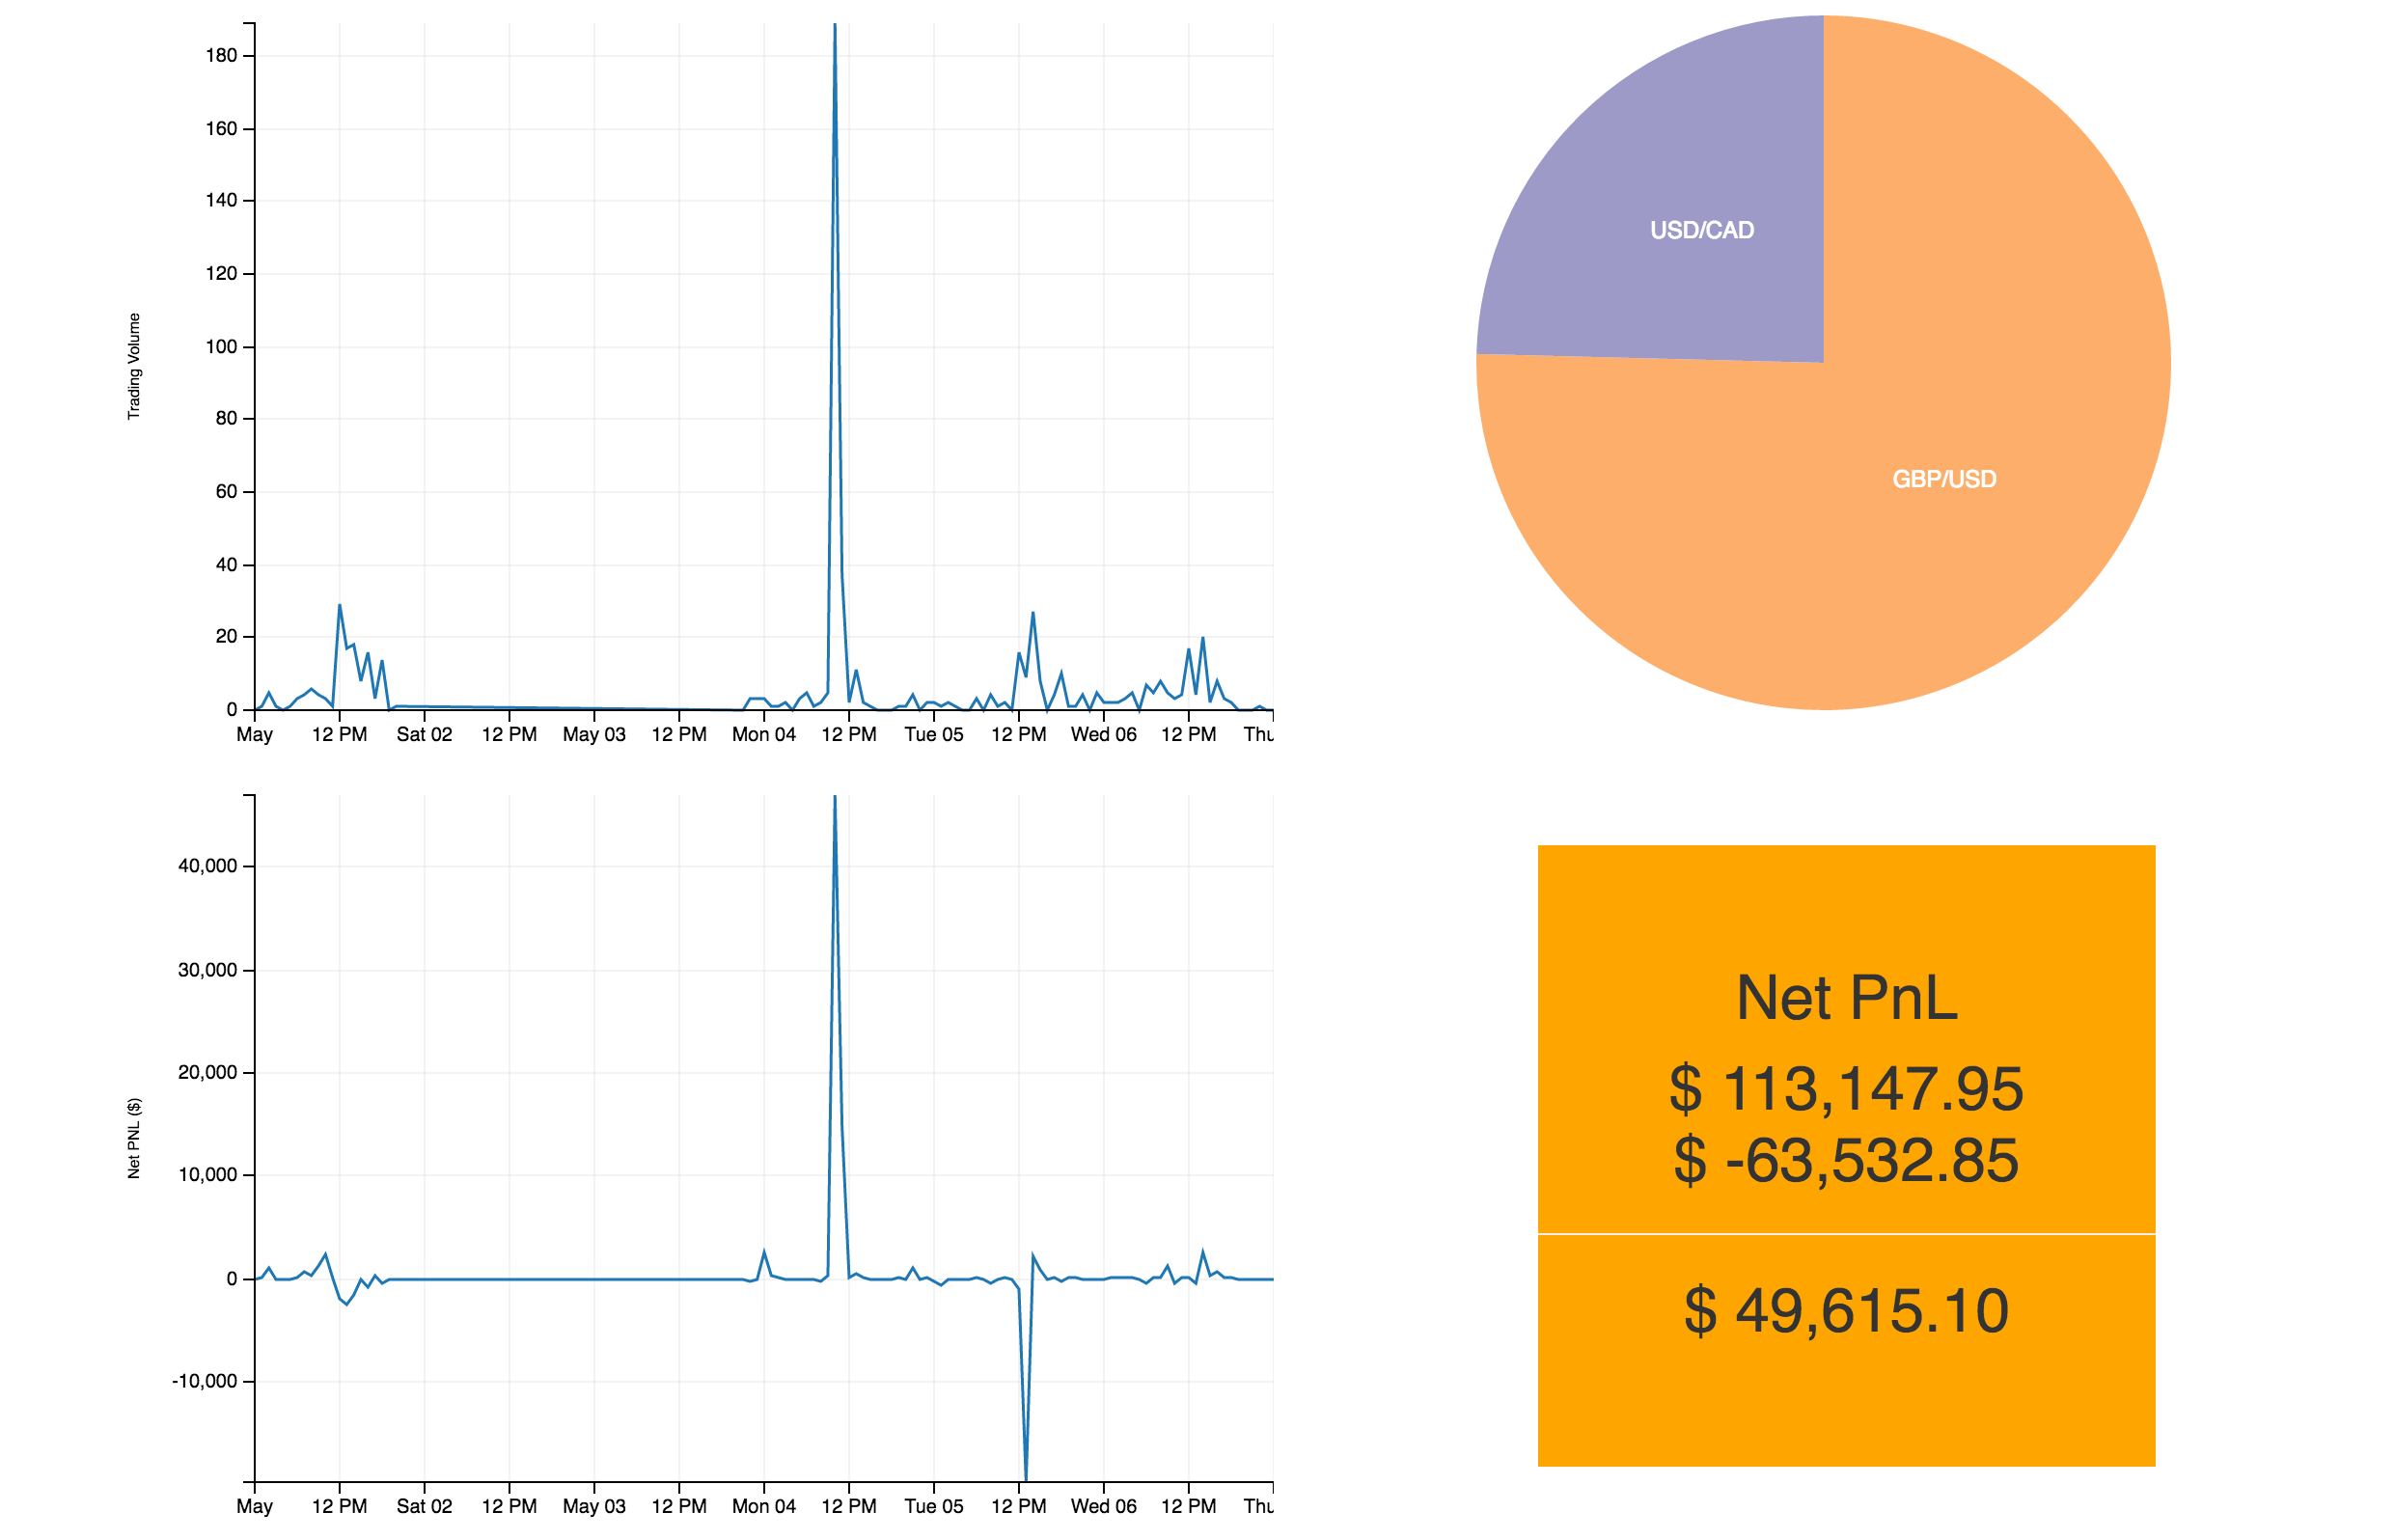
\includegraphics[width=\textwidth]{overview_1}
  \label{fig:overview_1}
\end{figure} 

\begin{figure}[H]
  \centering
  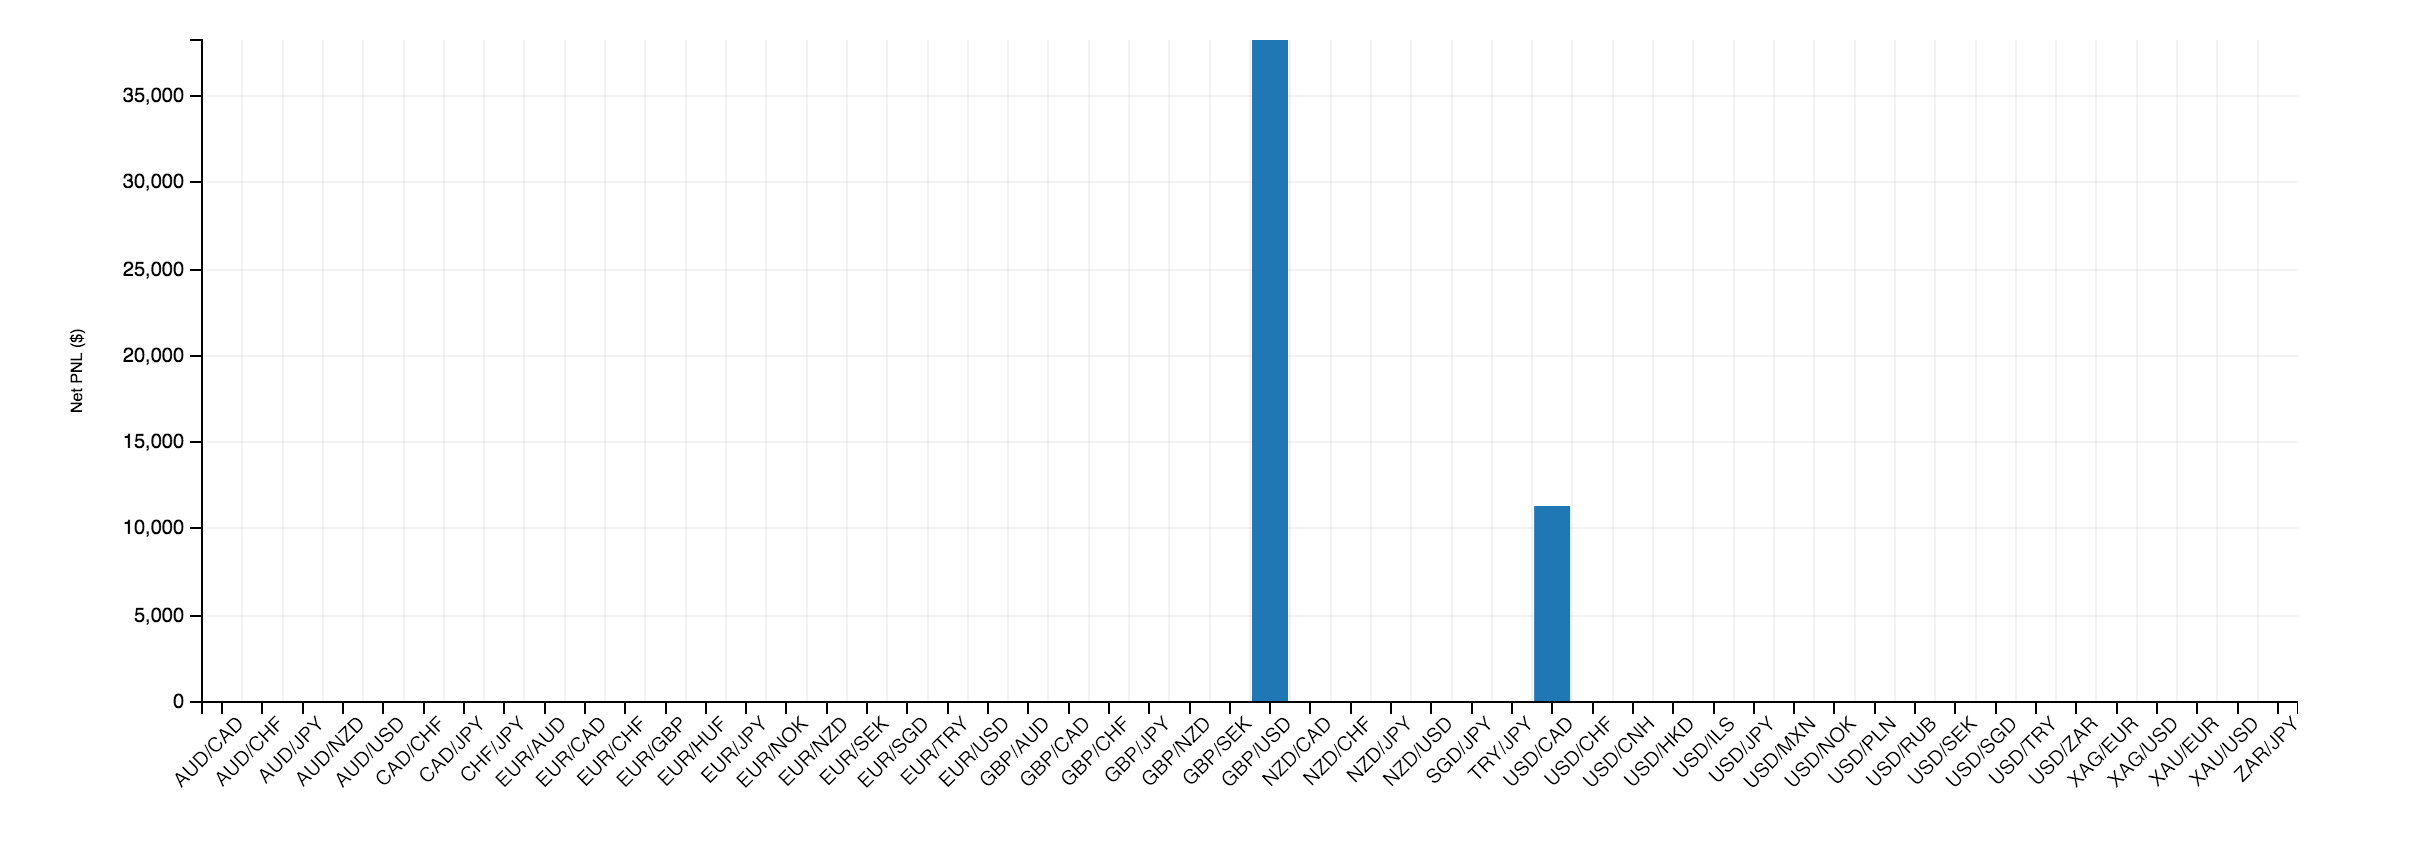
\includegraphics[width=\textwidth]{overview_2}
  \label{fig:overview_2}
\end{figure}

\begin{figure}[H]
  \centering
  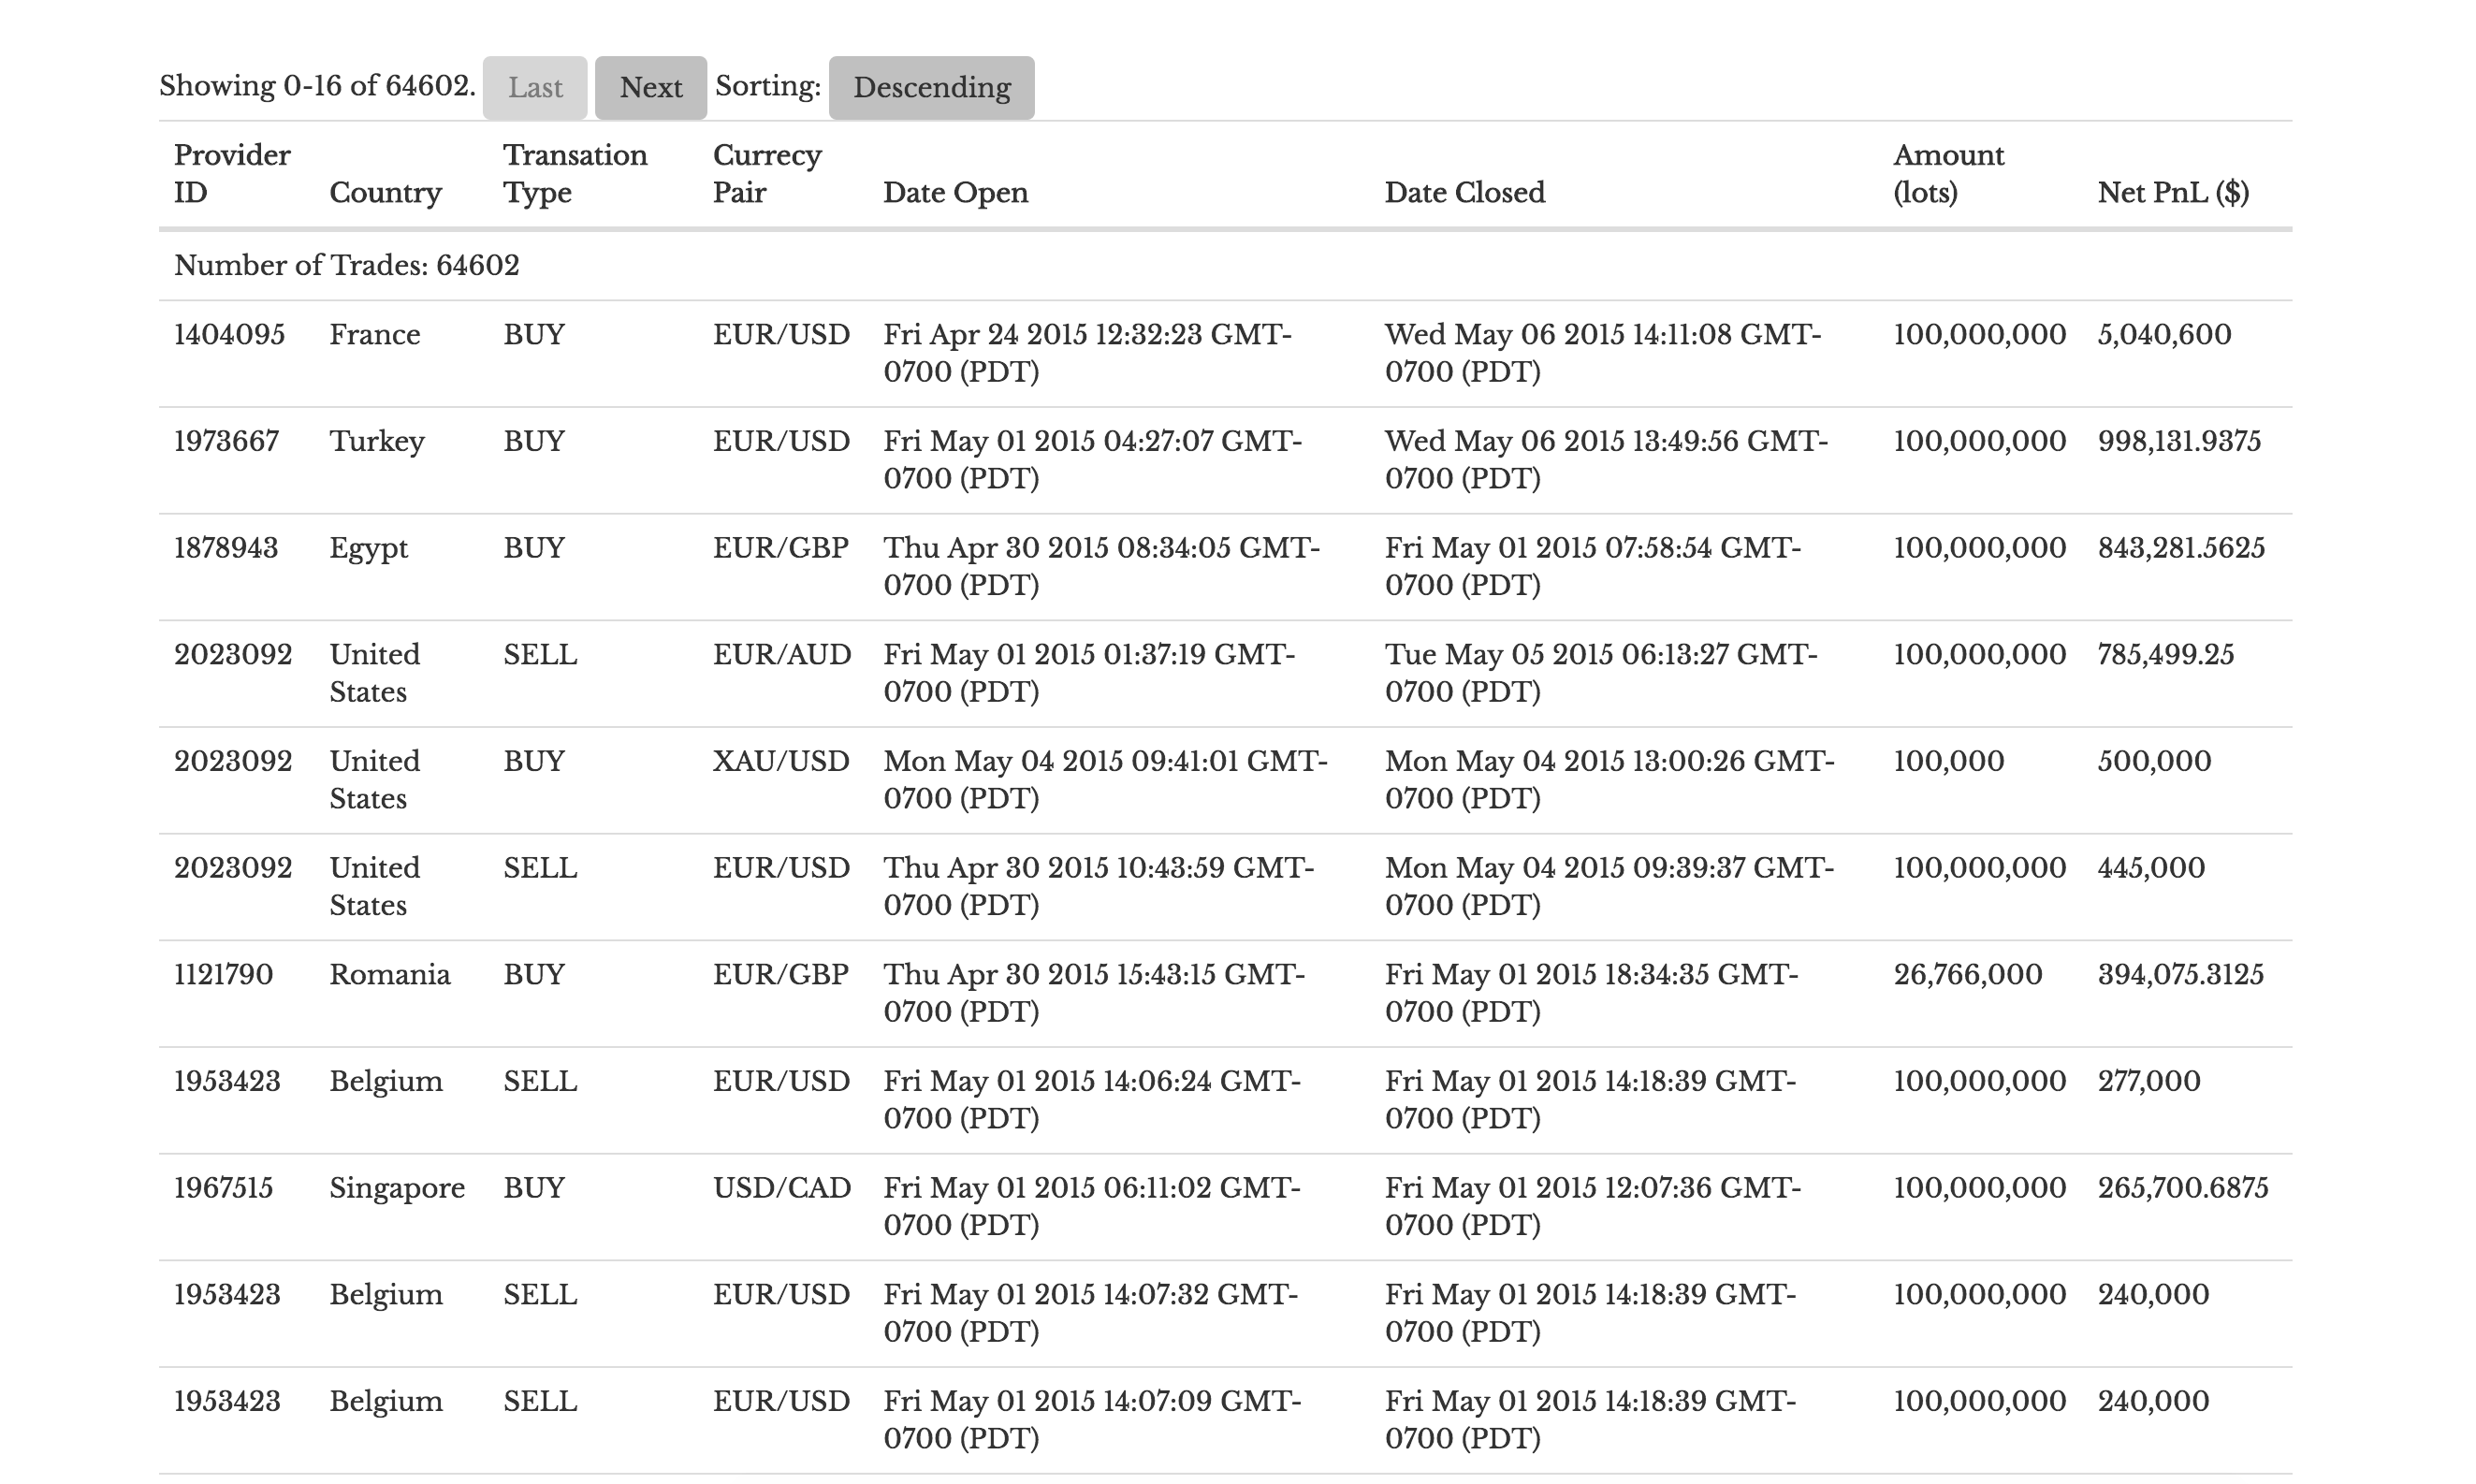
\includegraphics[width=\textwidth]{overview_3}
  \label{fig:overview_3}
\end{figure}

Τα διαγράμματα έχουν προσαρμοστεί και δείχνουν για παράδειγμα ποια ήταν τα νομισματικά ζεύγη που συναλλασσόταν αυτή τη στιγμή, πώς ήταν μοιρασμένα τα κέρδη και οι ζημιές ανά ζεύγος. Από τον πίνακα στο τέλος βλέπουμε ότι αυτή η αύξηση προήλθε κυρίως από μία κακή συναλλαγή ενός χρηματιστή που έχασε περίπου 5 εκατομμύρια δολάρια.

Έτσι μπορεί να δει οι συναλλαγές αυτές πότε έγιναν, ποιες ήταν επικερδείς και ποιες όχι, και πόσα χρήματα κινήθηκαν σ’ αυτές. Αντίστοιχα μπορεί να κάνει επιλογές πάνω σ’ αυτές τις απεικονίσεις και να δει πιο συγκεκριμένες πλευρές των δεδομένων του. 

Μ’ αυτό τον τρόπο μπορεί να αρχίσει να καταλαβαίνει ποια χαρακτηριστικά των συναλλαγών είναι πιο σημαντικά και μπορούν να χρησιμοποιηθούν για να εξαχθούν οι ψευδο-αξιολογήσεις. Για παράδειγμα: Ποια ζευγάρια βγάζουν το περισσότερο κέρδος; Oι συναλλαγές που έχουν μικρή διάρκεια – η διαφορά ανάμεσα στην ώρα ανοίγματος και κλεισίματος συναλλαγής – είναι καλύτερες ή χειρότερες; Τι σχέση παίζει ο αριθμός των συναλλαγών που γίνονται σε έναν ζεύγος;

Για παράδειγμα:

\begin{figure}[H]
	\centering
	\begin{minipage}{0.3\textwidth}
		\centering
		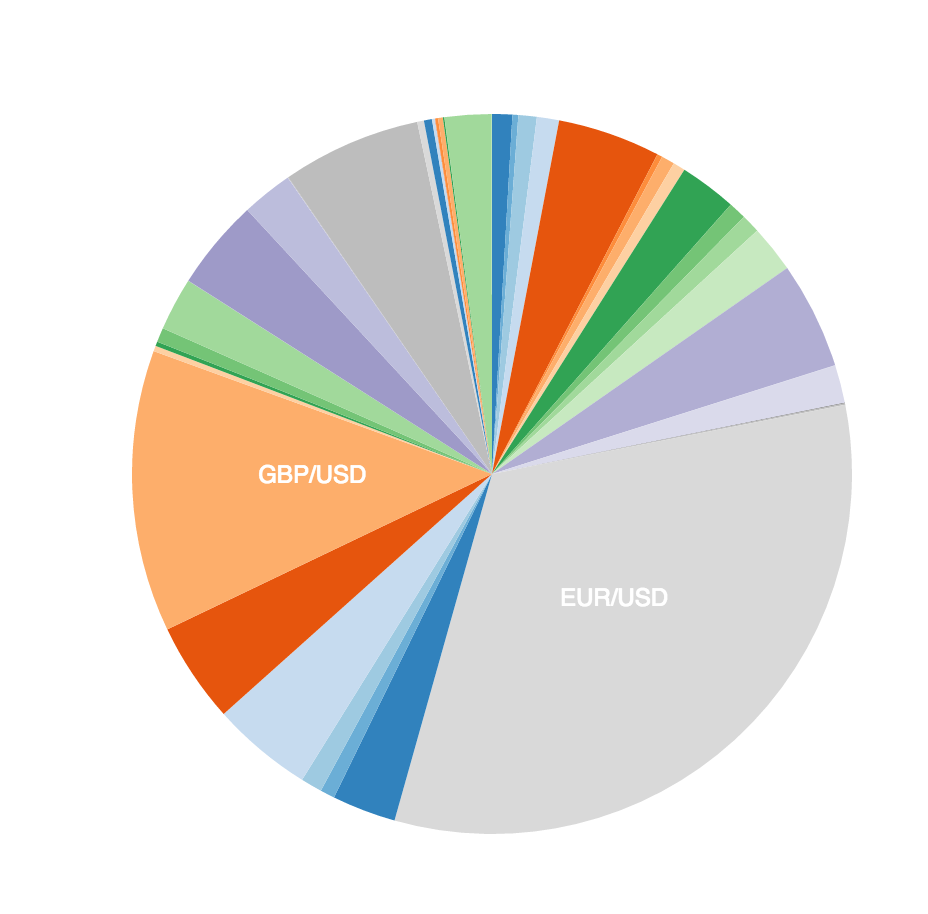
\includegraphics[width=\textwidth]{overview_4}
		\label{fig:overview_4}	
	\end{minipage}
	\hfill
	\begin{minipage}{0.7\textwidth}
		\centering
		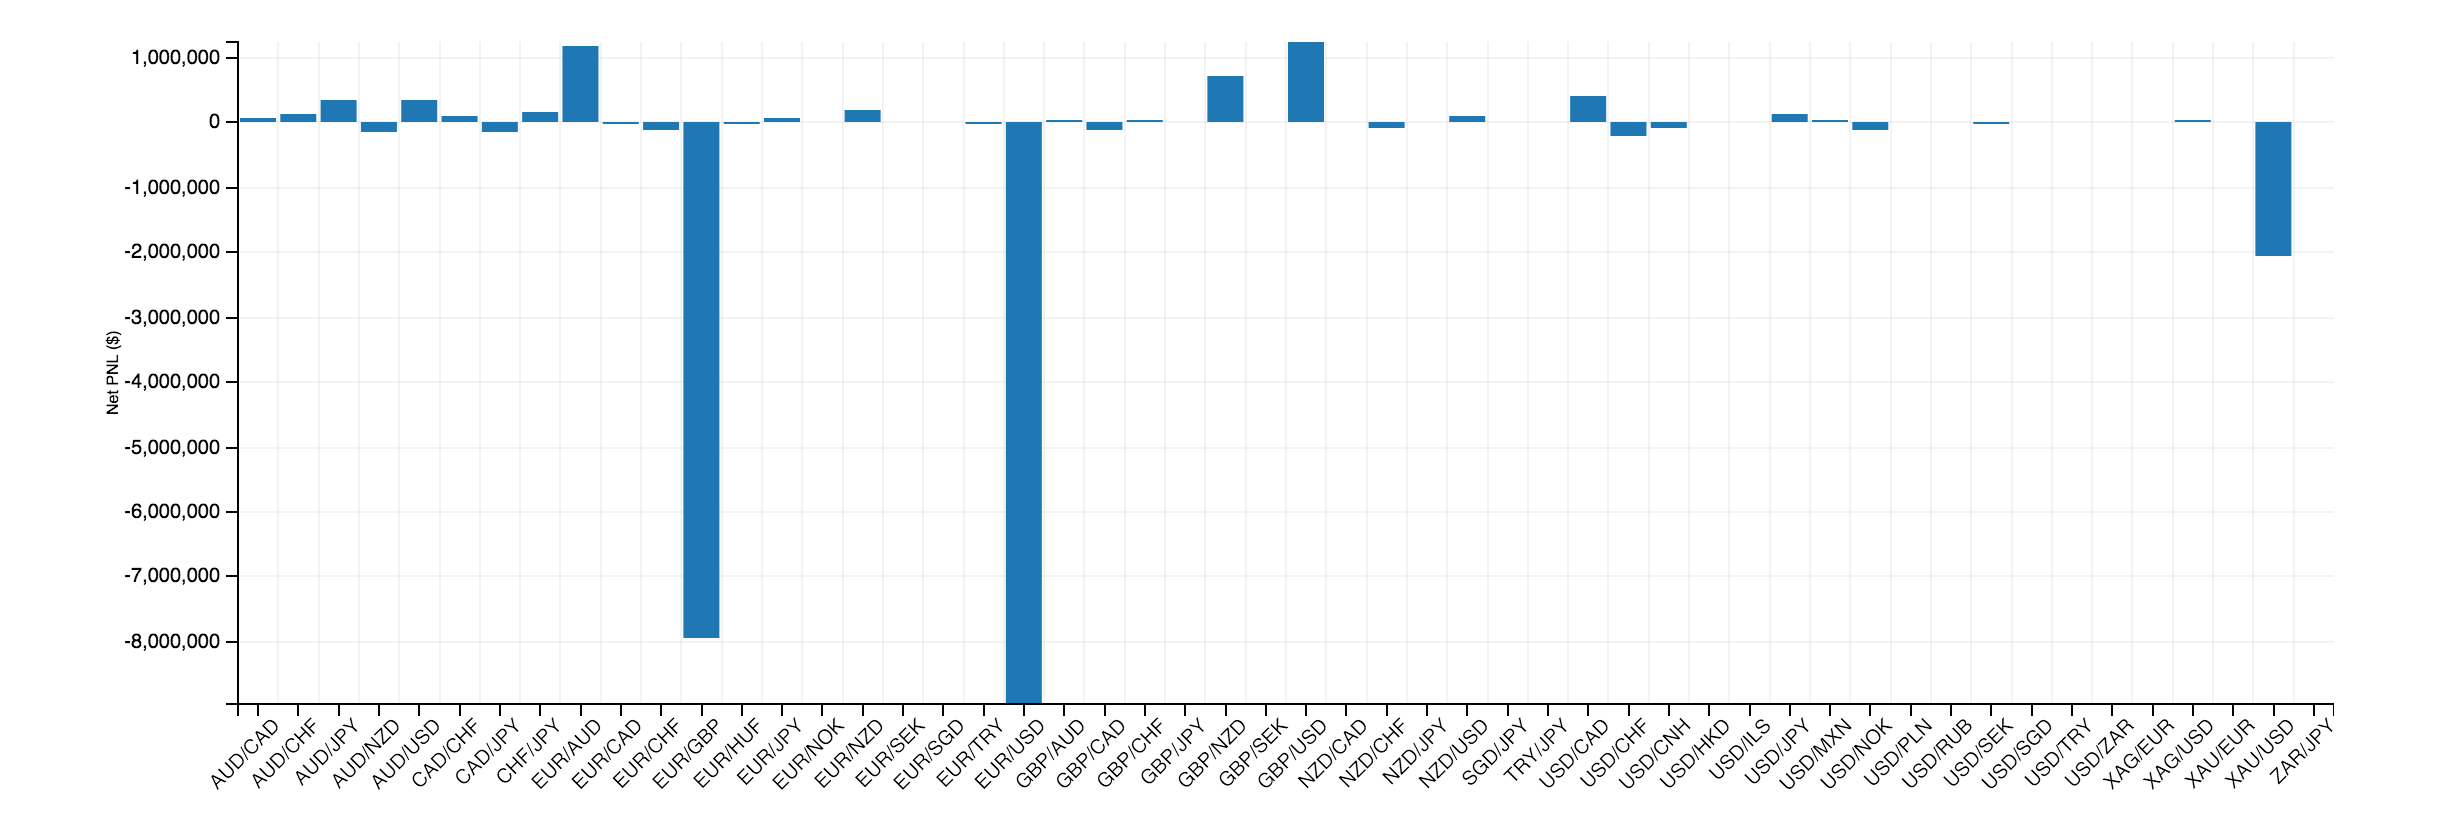
\includegraphics[width=\textwidth]{overview_5}
		\label{fig:overview_5}	
	\end{minipage}
\end{figure}

Βλέπουμε από το τελευταίο ραβδόγραμμα ότι τα ζεύγη που βγάζουν συνολικά το περισσότερο κέρδος αυτή την περίοδο είναι τα GBP/USD, EUR/AUD και GBP/NZD, ενώ οι περισσότερες ζημιές έχουν έρθει από τα EUR/USD, EUR/GBP και XAU/USD. Από την άλλη, τα ζεύγη που συναλλάχθηκαν περισσότερο είναι τα EUR/USD, GBP/USD, USD/JPY και EUR/JPY. Παρατηρούμε ότι παρόλο που το EUR/USD έχει τις περισσότερες ζημιές οι χρηματιστές το επιλέγουν τις περισσότερες φορές. Αν δούμε όμως αναλυτικά τις συναλλαγές και τις συγκρίνουμε μ’ αυτές του GBP/USD θα δούμε ότι στο EUR/USD οι καλύτερες συναλλαγές έχουν σημαντικά περισσότερα κέρδη απ’ ότι στο GBP/USD. Αυτό μας δείχνει ότι τα κέρδη (PnL) δεν μπορεί να είναι το αποκλειστικό χαρακτηριστικό για την αξιολόγηση μίας συναλλαγής. Ο αριθμός των συναλλαγών (Trade Count) μπορεί να περιέχει περισσότερη πληροφορία, γιατί ο χρηματιστής που έχει απ’ ευθείας γνώση της αγοράς επέλεξε συνειδητά να συναλλαχθεί το νομισματικό ζεύγος. Έτσι στη συνέχεια επιλέγουμε ως χαρακτηριστικά το Net PnL και το Trade Count μαζί με το Trade Duration.

\section{Επιλογή Χαρακτηριστικών – Feature Selection}

Αφού ο προγραμματιστής καταλήξει στα χαρακτηριστικά που θα χρησιμοποιήσει μπορεί να τα υλοποιήσει προγραμματιστικά και στη συνέχεια να τα δώσει πίσω στο Visfx ώστε να τα οπτικοποιήσει. 

Στη δικιά μας ανάλυση χρησιμοποιήσαμε τέσσερεις ομάδες χαρακτηριστικών: χαρακτηριστικά ανά συναλλαγή, ανά χρηματιστή, ανά νόμισμα, και ανά χώρα. Σε κάθε μία απ’ αυτές τις ομάδες χρησιμοποιήσαμε τα εξής χαρακτηριστικά: τον αριθμό των συναλλαγών, τη διάρκεια της συναλλαγής, το καθαρό κέρδος ή ζημιά (Net PnL – Profits and Losses), το συνολικό ποσό που συναλλάχθηκε και τον λόγο των κερδών προς αυτό το ποσό.

Εδώ ερχόμαστε στη δεύτερη καρτέλα του Visfx όπου μπορούμε να δούμε πως συμπεριφέρονται τα χαρακτηριστικά που επιλέξαμε. Πάλι, ο χρήστης μπορεί να φιλτράρει τα χαρακτηριστικά βάση διαφόρων παραγόντων και αντίστοιχα να δει τις απεικονίσεις.

\begin{figure}[H]
  \centering
  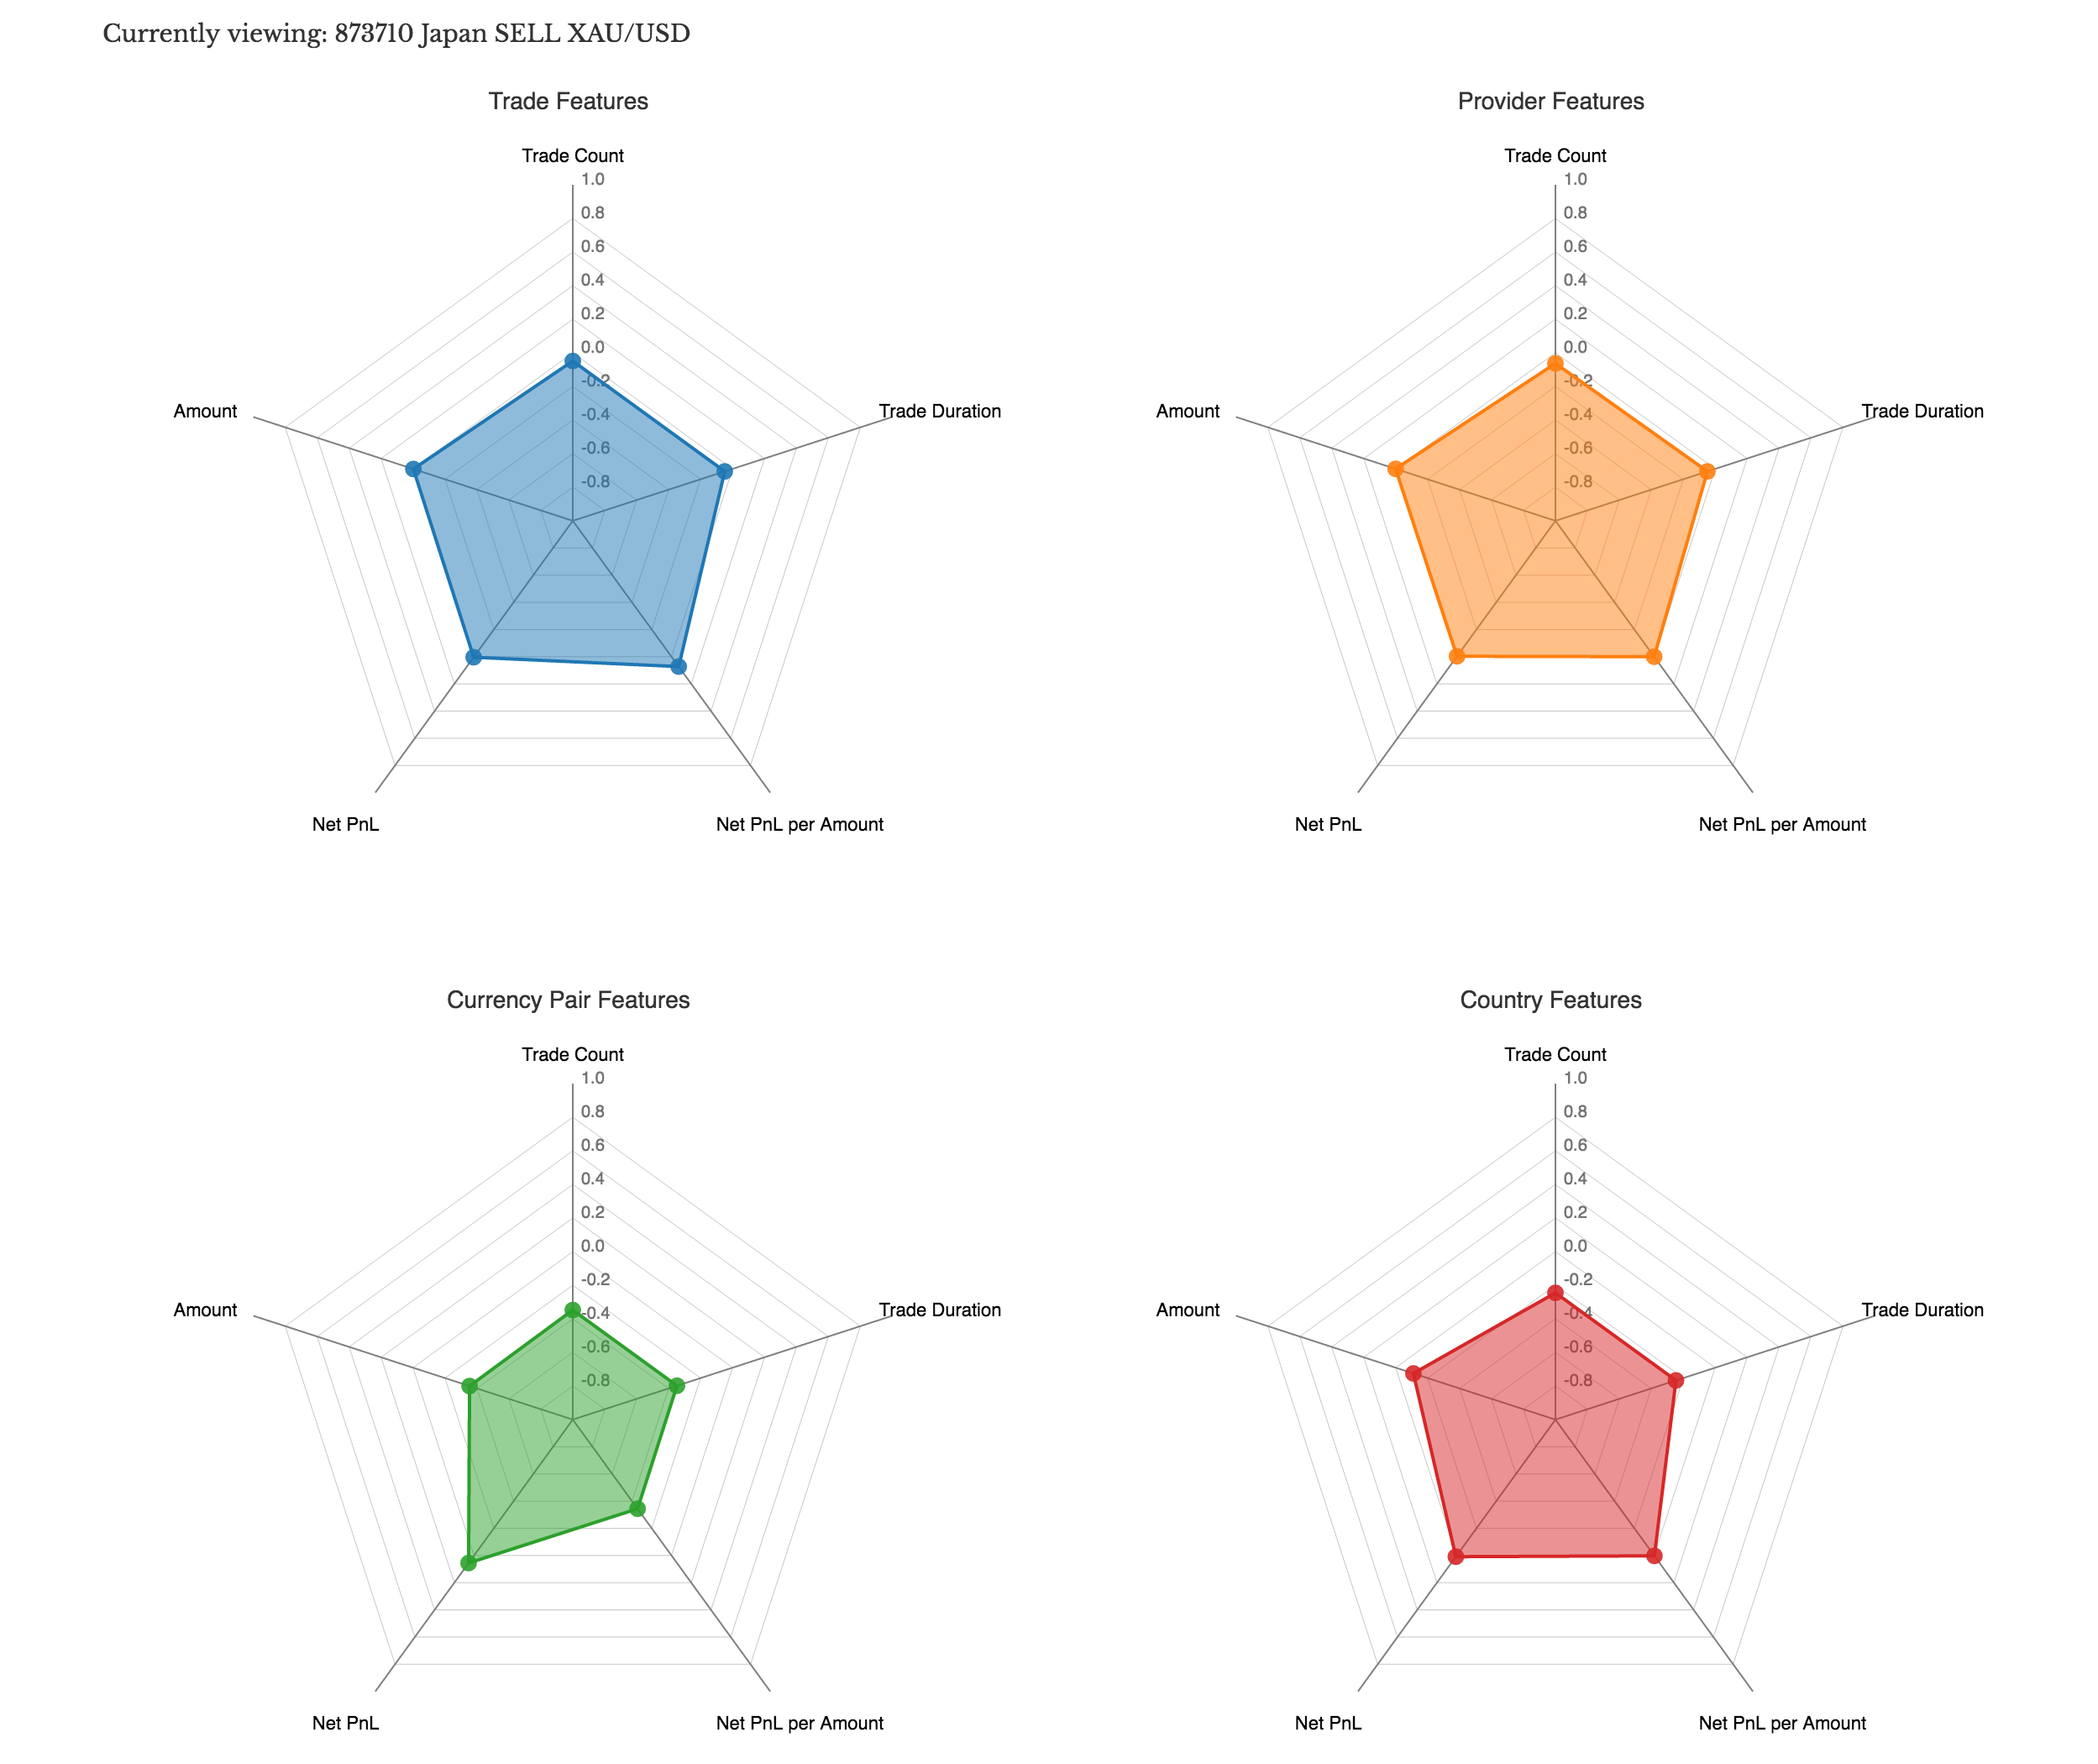
\includegraphics[width=\textwidth]{features_1}
  \label{fig:features_1}
\end{figure}

Παραπάνω βλέπουμε τις κανονικοποιημένες τιμές των χαρακτηριστικών που επιλέξαμε για μια συγκεκριμένη συναλλαγή. Βλέπουμε ότι η συγκεκριμένη συναλλαγή βρίσκεται στον κοντά στο μέσο όρο στα περισσότερα χαρακτηριστικά της, όπως το ίδιο συμβαίνει και με τον συγκεκριμένο χρηματιστή. Από την άλλη βλέπουμε ότι το Ασήμι συναλλάσσεται λίγες φορές (trade count κάτω από τον μέσο όρο) αλλά έχει κέρδη πάνω από τον μέσο όρο. Ενώ για την χώρα, στην περίπτωσή μας η Ιαπωνία, κάνει λιγότερες συναλλαγές από τον μέσο όρο, αλλά και οι συναλλαγές που κάνουν οι χρηματιστές από αυτή τη χώρα έχουν σημαντικά μικρότερη διάρκεια από το μέσο όρο.

Πέρα από τις διαισθήσεις που μπορούμε να αποκτήσουμε πάνω στα δεδομένα μας – ο οποίες μπορούν να χρησιμοποιηθούν σαν ανάδραση για να επιλέξουμε ποια από τα χαρακτηριστικά που διαλέξαμε θα κρατήσουμε ή θα αλλάξουμε – μελετώντας πως συμπεριφέρονται τα οι τιμές των χαρακτηριστικών στις διάφορες συναλλαγές, χρηματιστές, νομίσματα ή χώρες μπορούμε να σκεφτούμε πως θα τις συνδυάσουμε ώστε να βγάλουμε την ψευδο-αξιολόγηση για κάθε συναλλαγή.

Ξανά, στη δικιά μας ανάλυση, επιλέξαμε να μην κρατήσουμε το χαρακτηριστικό Amount, γιατί παρατηρήσαμε ότι είχε μεγάλη διακύμανση ή οποία όμως δεν ήταν σχετική με την ποιότητα της συναλλαγής—γι’ αυτό το λόγο πετάξαμε και το χαρακτηριστικό Net PnL per Amount. 

Αφού επιλέξουμε ποια χαρακτηριστικά θα κρατήσουμε μπορούμε να δούμε πως αυτά συμπεριφέρονται στο σύνολο των συναλλαγών μας. Αφού περάσουμε τις τιμές των χαρακτηριστικών για κάθε συναλλαγή στο Visfx, τρέχουμε το Spark script points.py και εξάγουμε την MDS χωρική απεικόνιση των δεδομένων μας βάση τα επιλεγμένα χαρακτηριστικά. Επίσης μπορούμε να δώσουμε τα βάρη που επιλέξαμε (στη δική μας ανάλυση βγήκαν από τη μέθοδο PCA) και να δούμε με χρώμα πώς κινούνται οι ψευδο-αξιολογήσεις στις συναλλαγές μας. Η κλίμακα είναι από το 0 στο 5 και από το κόκκινο στο μπλε.

\begin{figure}[H]
  \centering
  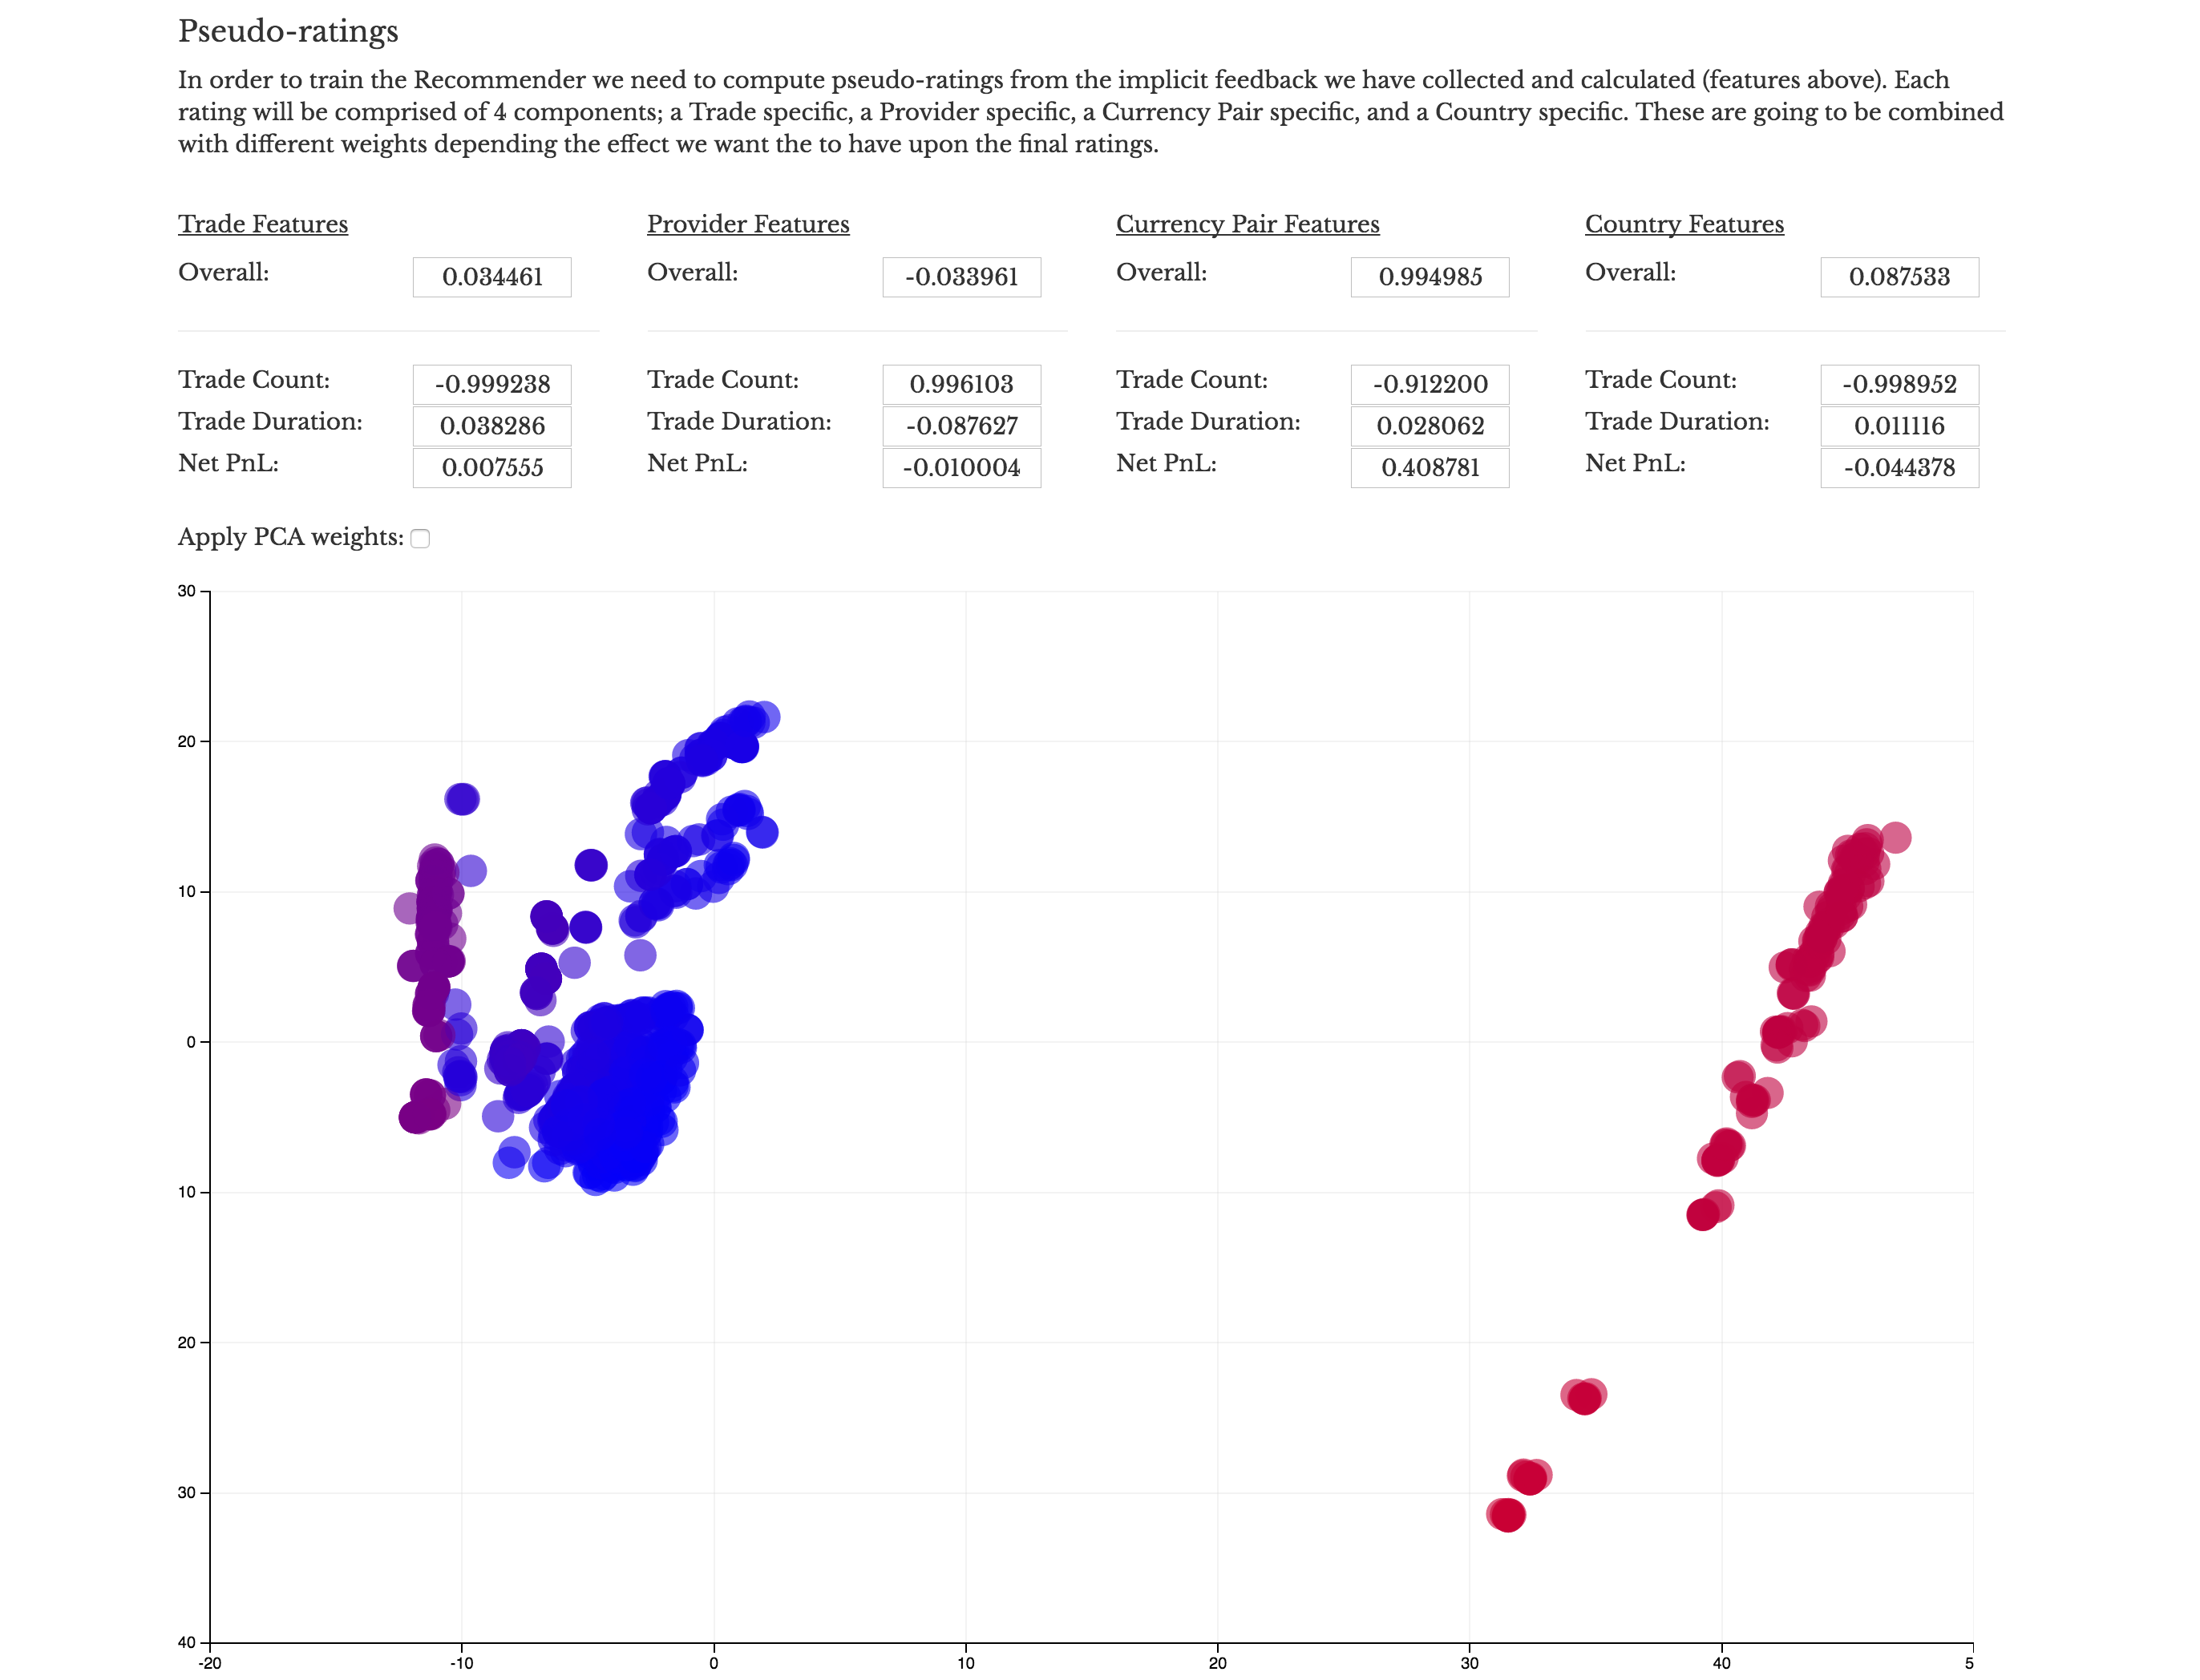
\includegraphics[width=\textwidth]{features_2}
  \label{fig:features_2}
\end{figure}

Εδώ μπορούμε αμέσως να δούμε ότι δημιουργούνται διάφορες ομάδες στις συναλλαγές μας οποίες βαθμολογούνται επίσης διαφορετικά. Έχοντας από τις προηγούμενες απεικονίσεις αποκτήσει γνώση των δεδομένων μας μπορούμε να αξιολογήσουμε αν οι συγκεκριμένες συναλλαγές (που φέρνοντας το ποντίκι πάνω σε κάθε σημείο μπορούμε να δούμε λεπτομέρειες γι’ αυτό) έχουν βαθμολογηθεί σωστά και αμέσως να κάνουμε αλλαγές στον τρόπο υπολογισμού των ψευδο-αξιολογήσεων. Ακόμα αλλάζοντας τις επιλογές στην κορυφή της σελίδα μπορούμε να φιλτράρουμε τα σημεία που εμφανίζονται στο MDS διάγραμμα. 

\begin{figure}[H]
  \centering
  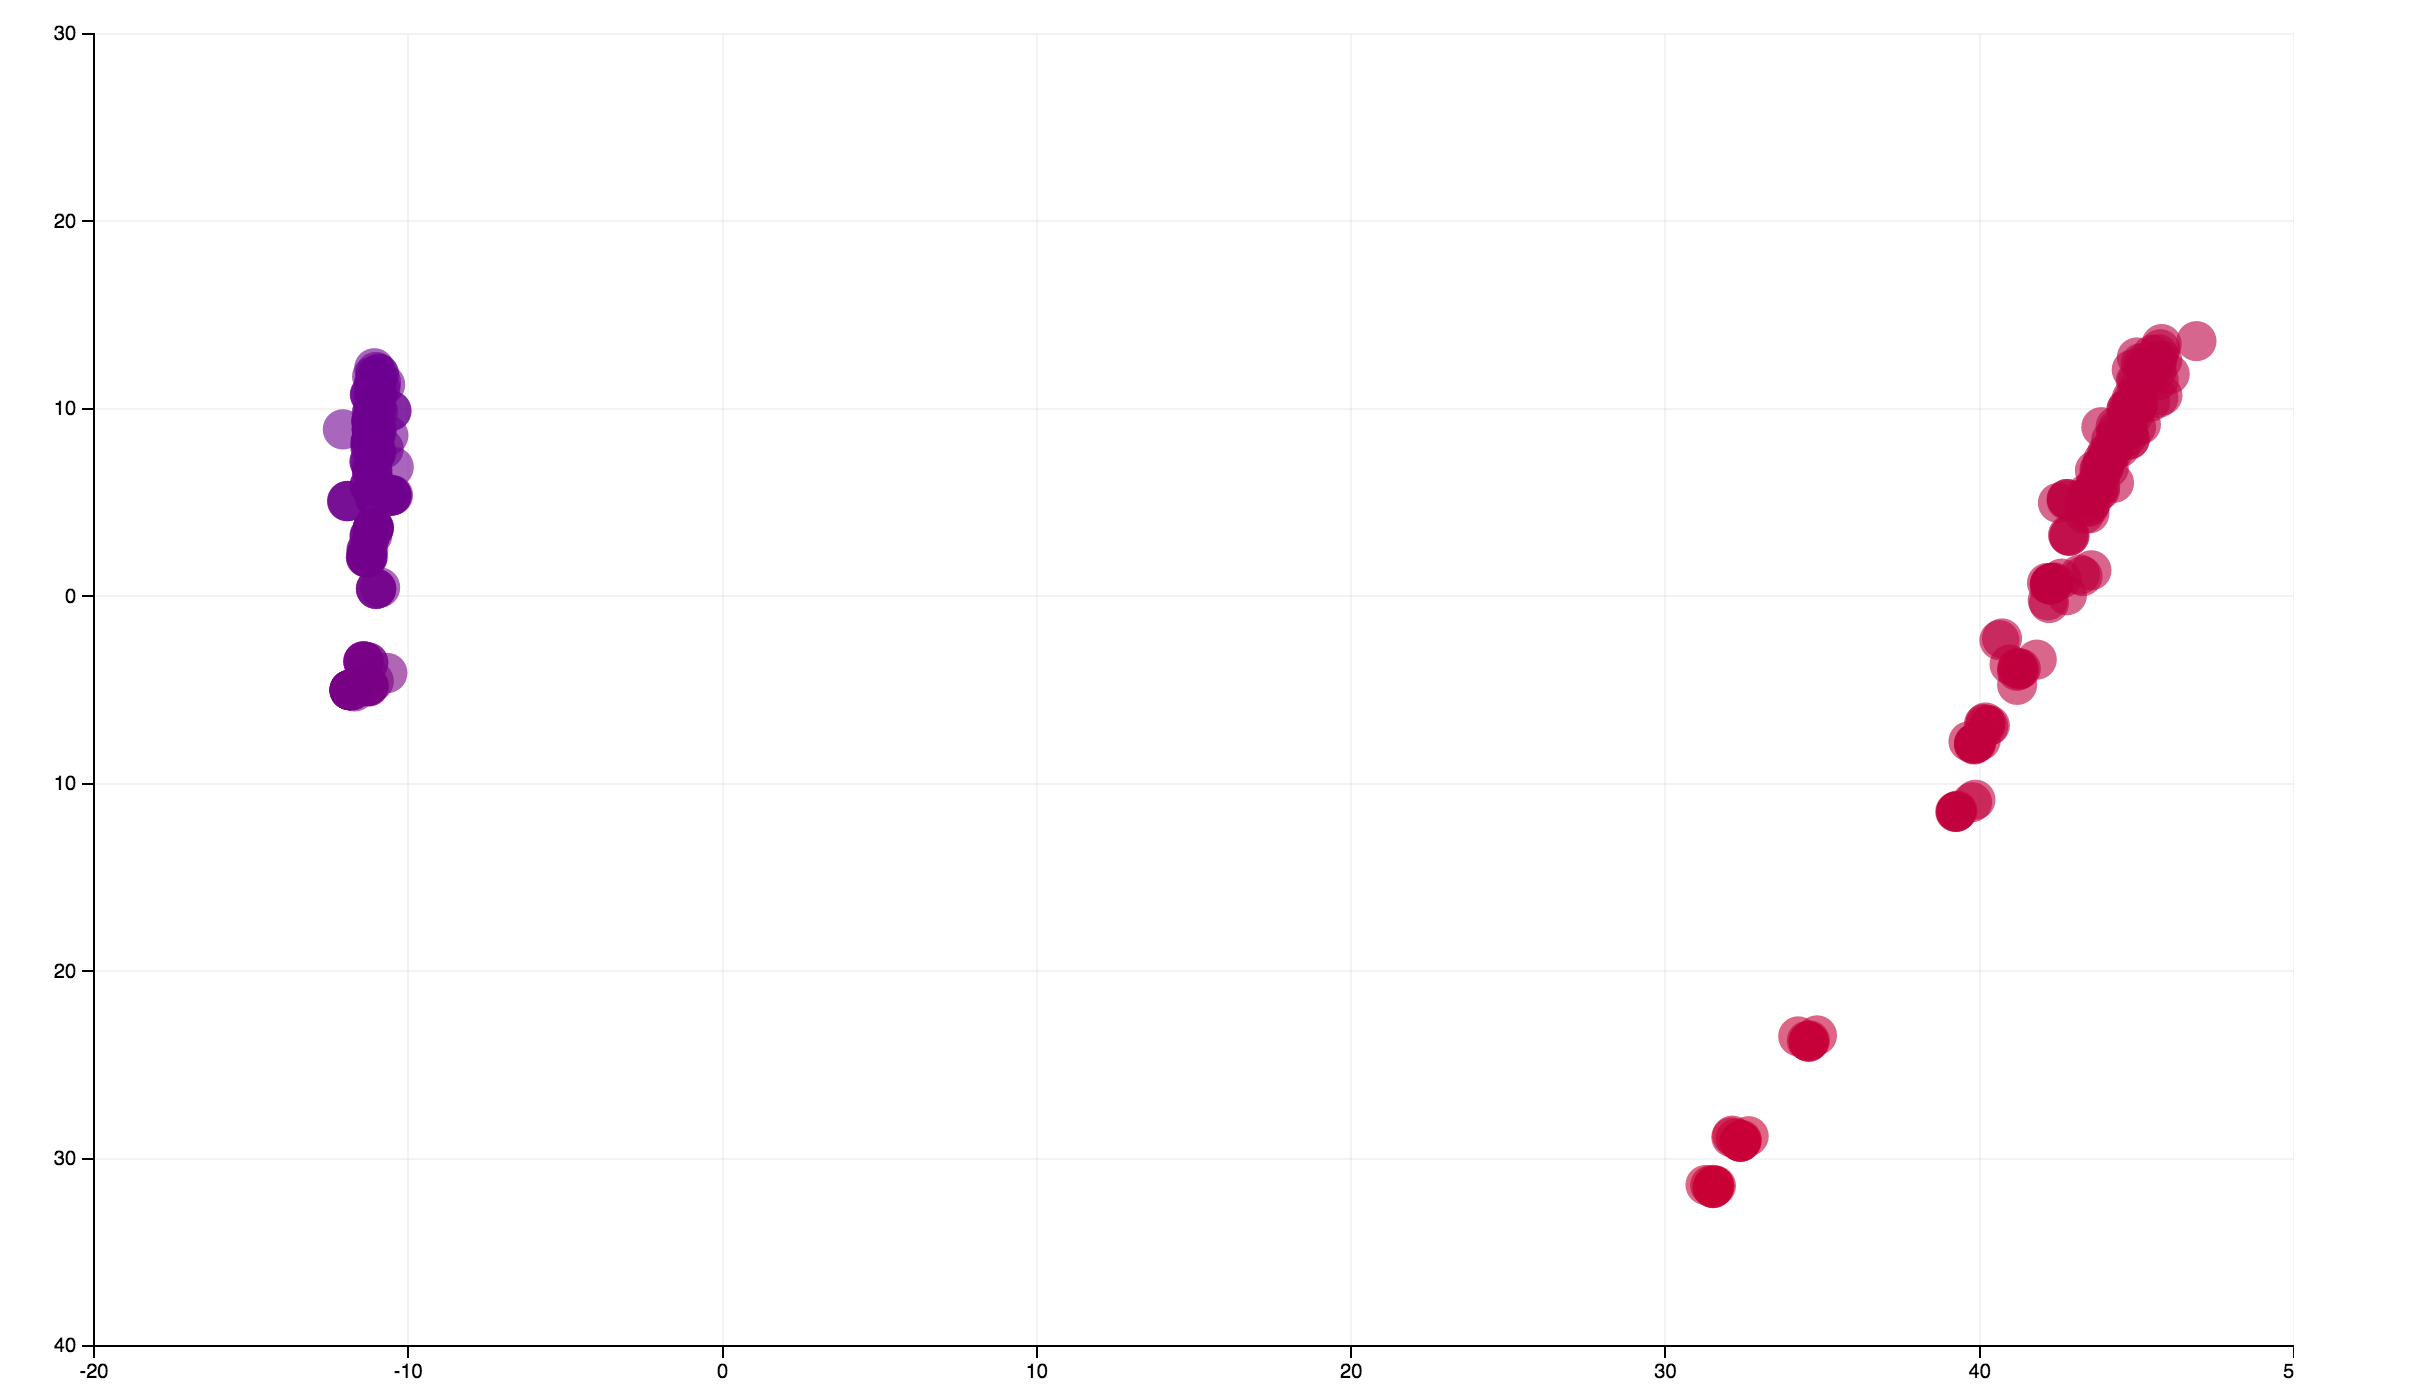
\includegraphics[width=\textwidth]{features_3}
  \label{fig:features_3}
\end{figure}

Παραπάνω φαίνονται οι συναλλαγές που έκαναν χρηματιστές στο ζεύγος EUR/USD και παρακάτω στο GBP/USD

\begin{figure}[H]
  \centering
  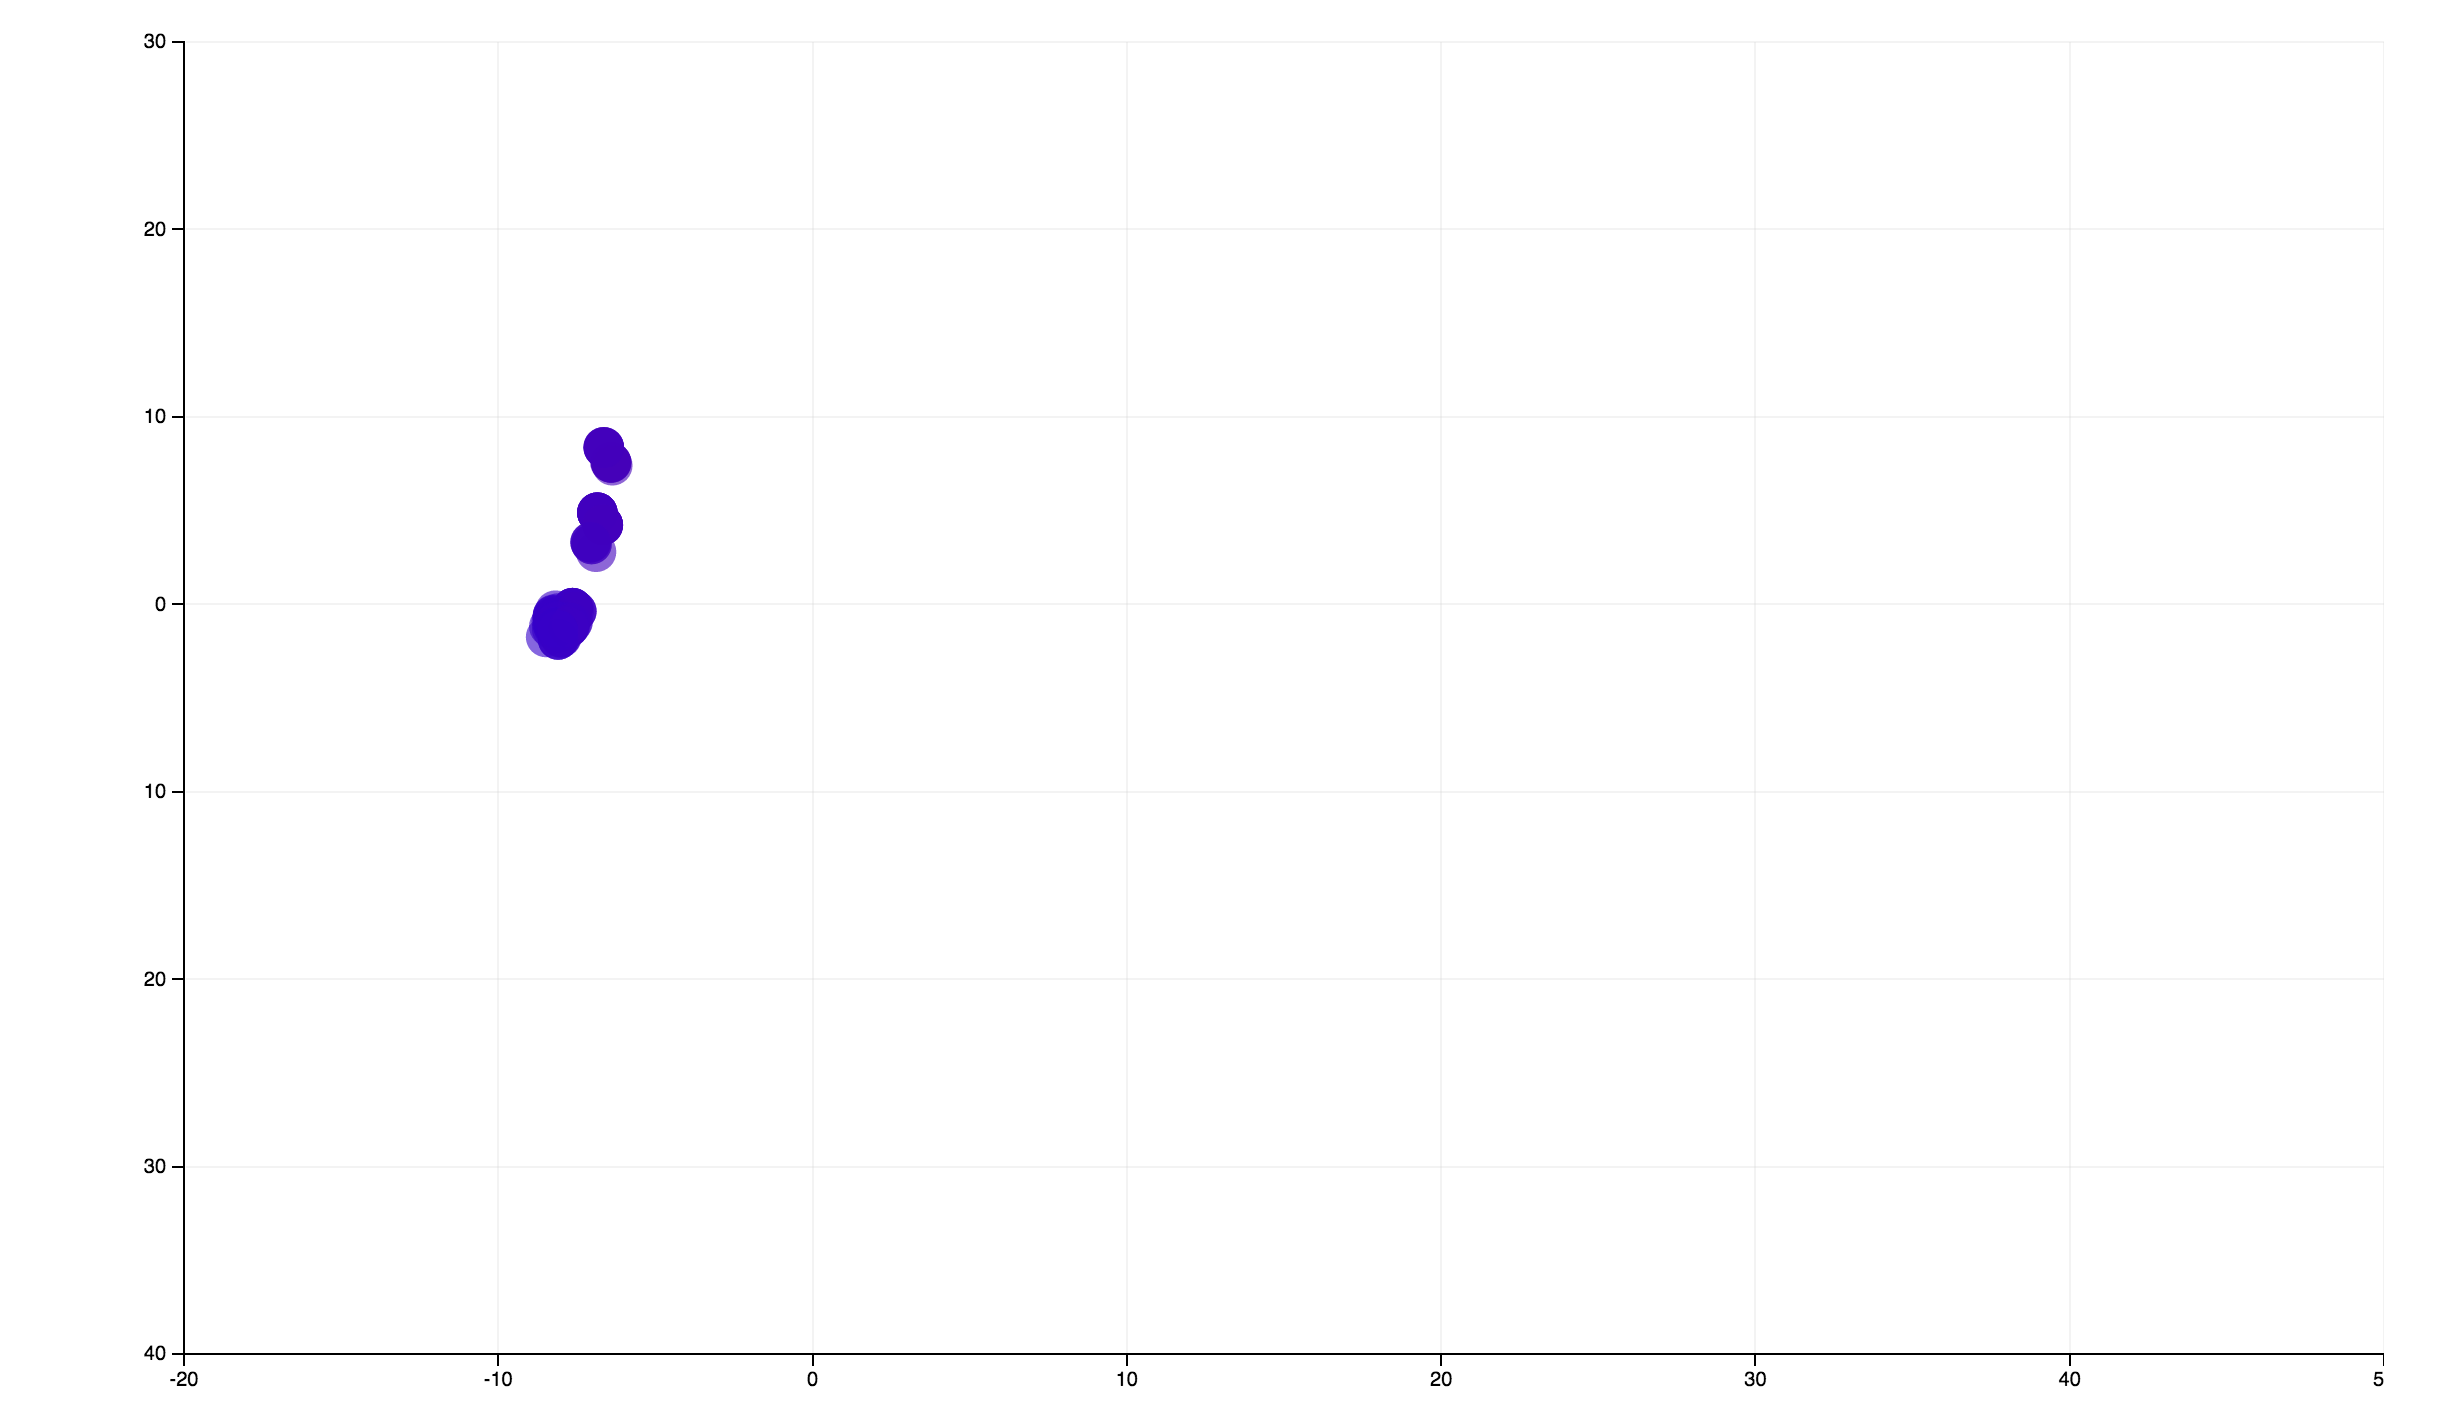
\includegraphics[width=\textwidth]{features_4}
  \label{fig:features_4}
\end{figure}

Παρατηρείται γενικά το φαινόμενο λόγω των ζημιών ότι το EUR/USD βαθμολογείται χαμηλά (κόκκινα και μοβ σημεία) ενώ από την άλλη το GBP/USD βαθμολογείται υψηλά λόγω της δημοφιλίας του και των κερδών του. Έτσι δημιουργείται ένας βρόχος οπτικής ανάδρασης, όπου οι αλλαγές στον τρόπο υπολογισμού των ψευδο-αξιολογήσεων είναι άμεσα εμφανείς και μπορούμε άμεσα να πάρουμε αποφάσεις. Για παράδειγμα αν είχαμε χρησιμοποιήσει διαφορετικά βάρη και αντί το χαρακτηριστικό Net PnL το Net PnL per Amount θα είχαμε τα ακόλουθα αποτελέσματα:

\begin{figure}[H]
  \centering
  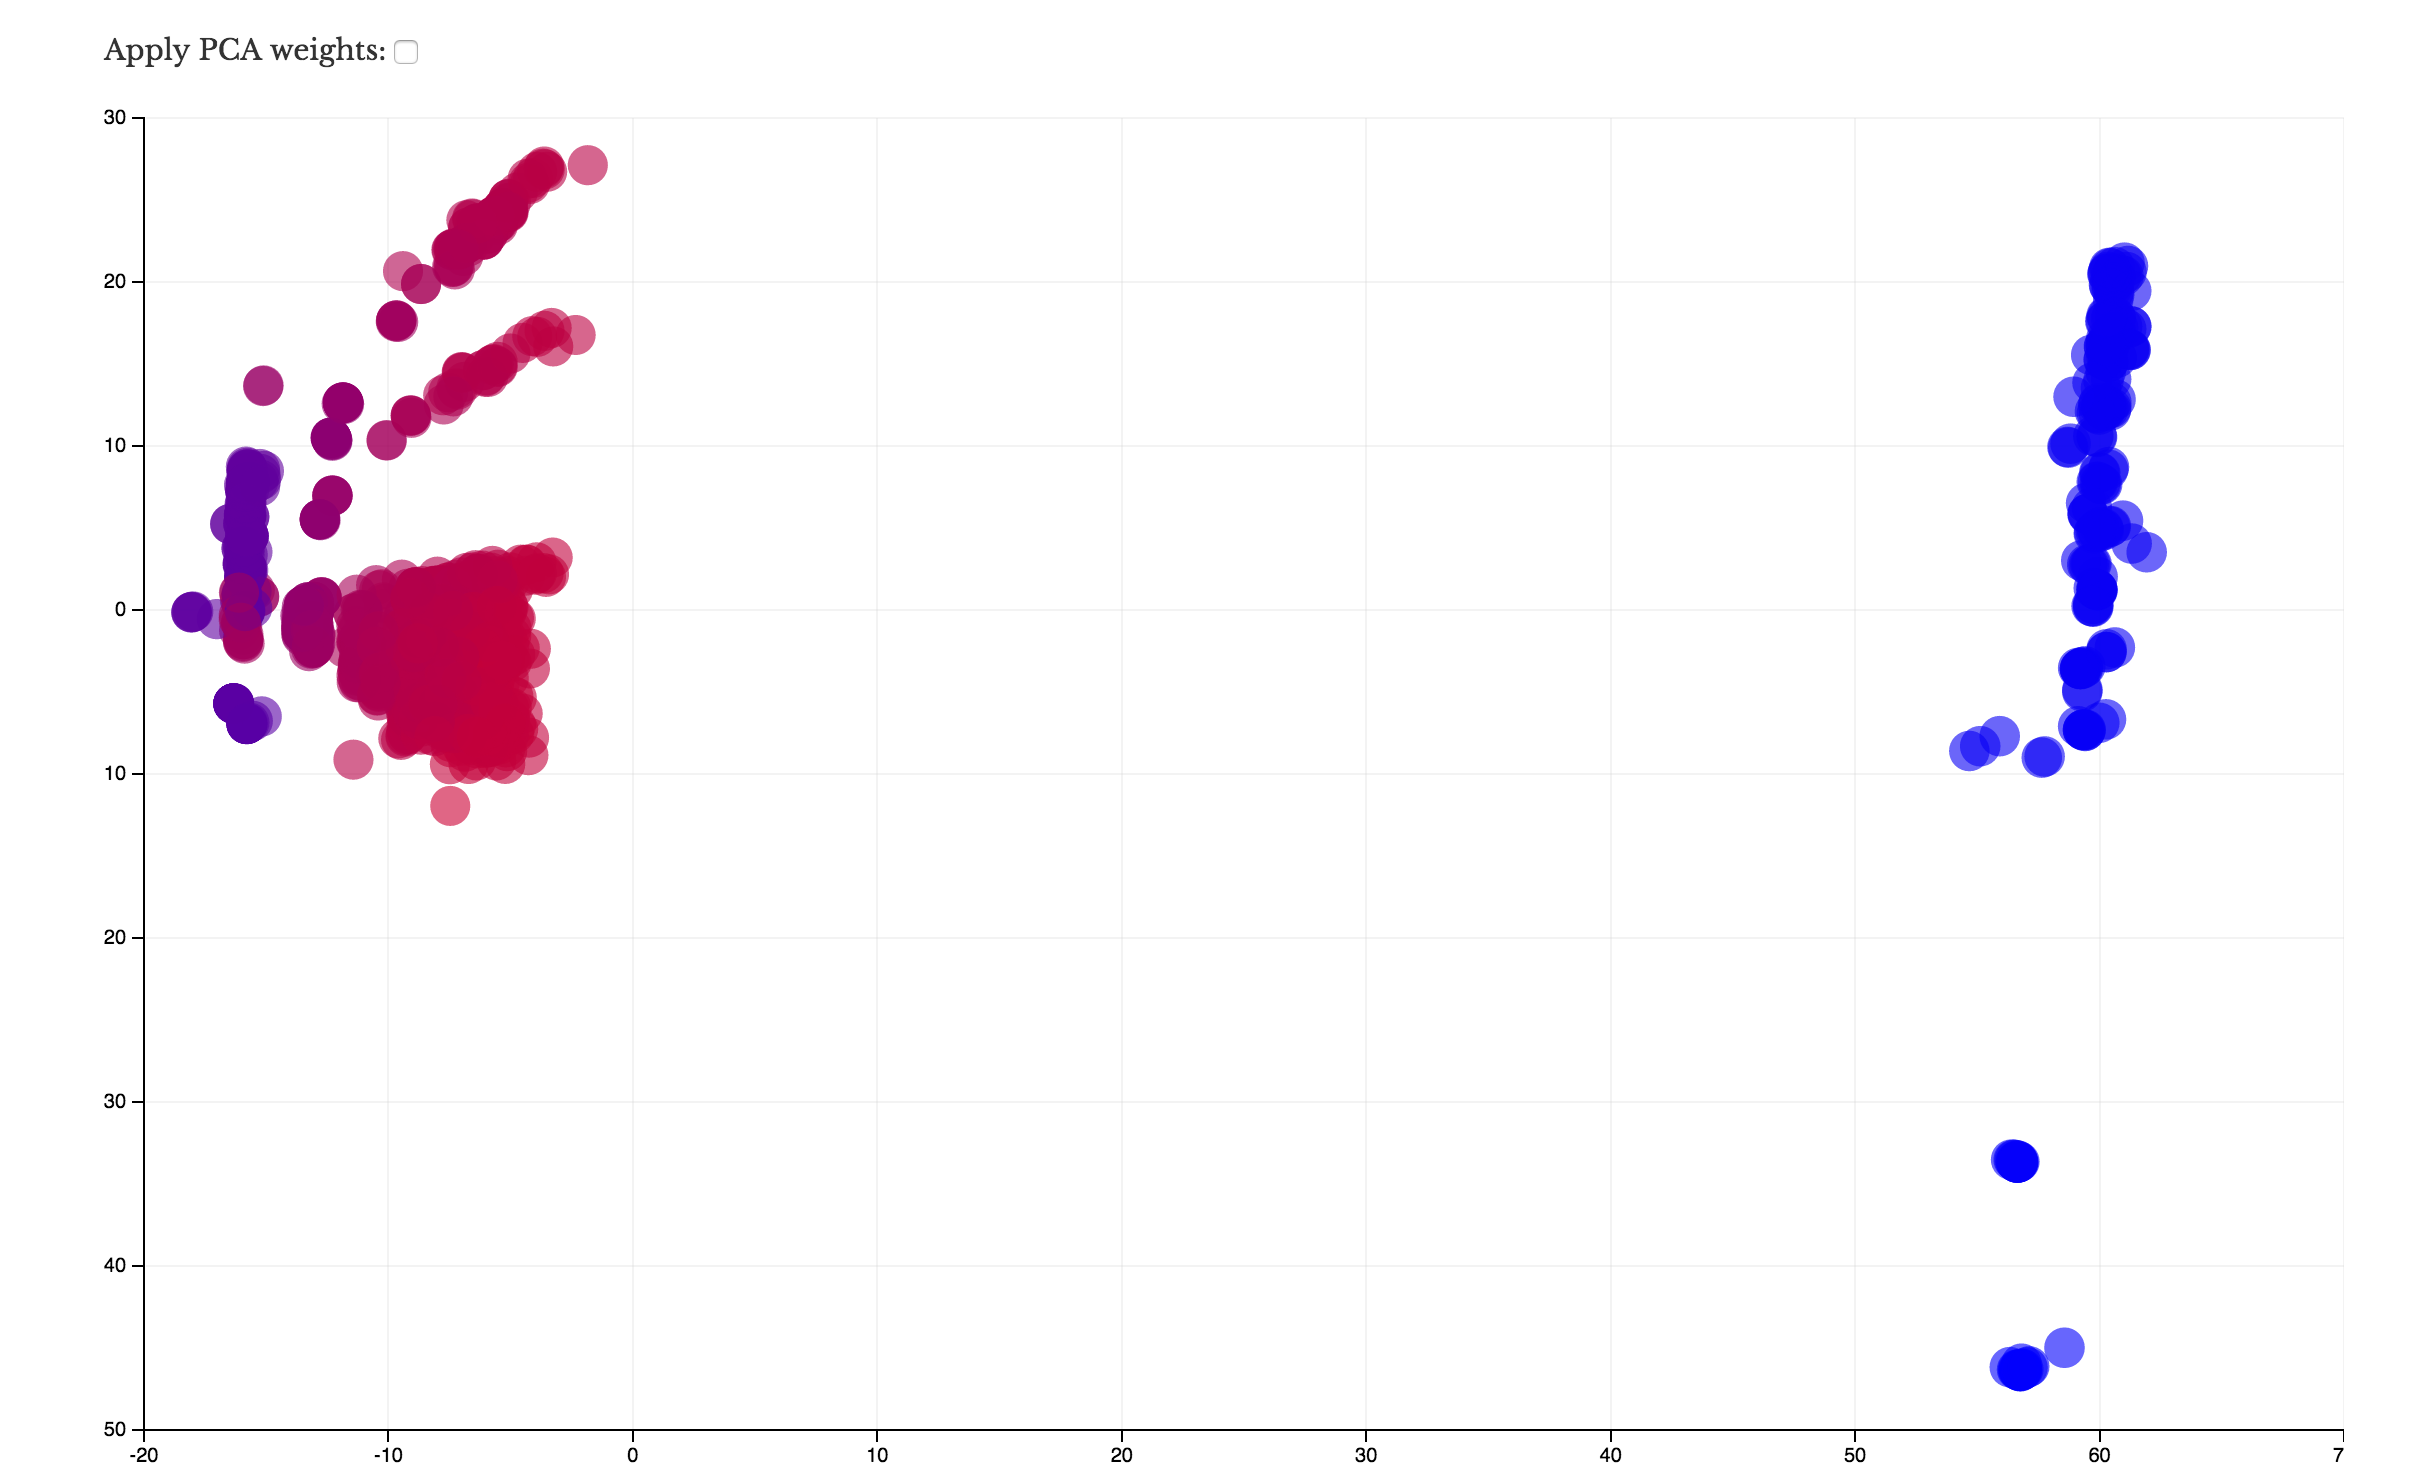
\includegraphics[width=\textwidth]{features_5}
  \label{fig:features_5}
\end{figure}

Αυτό είναι ένα σενάριο το οποίο είχα αρχικά χρησιμοποιήσει αλλά τελικά απορρίψει. Όπως βλέπουμε και στο διάγραμμα, οι συναλλαγές EUR/USD έχουν βαθμολογηθεί υπέρμετρα υψηλότερα από όλες τις υπόλοιπες. Αυτό συνέβη γιατί όπως είδαμε και στην ανάλυση των δεδομένων το ζεύγος αυτό είναι πολύ δημοφιλές, οι χρηματιστές το συναλλάσουν πολλές φορές και βάζουν αντίστοιχα μεγάλα ποσά (amount), αλλά όχι αντίστοιχα κερδοφόρο. Επίσης λόγω της φύσης του αλγορίθμου η δημοφιλία ενός ζεύγους λαμβάνεται ήδη υπόψιν συνεπώς δε θέλουμε να του δώσουμε υπέρμετρα υψηλή αξιολόγηση.

\section{Παρουσίαση Συστάσεων}

Τέλος έχοντας καταλήξει στον τρόπο υπολογισμού των ψευδο-αξιολογήσεων, μπορούμε να τρέξουμε το RS και να αξιολογήσουμε τις επιδόσεις του. Αυτό γίνεται στην τρίτη και τελευταία καρτέλα του Visfx, Recommendations. Εδώ μπορούμε να δούμε μία άμεση επισκόπηση των συστάσεων που δίνουμε στους χρηματιστές μέσω ενός Parallel Coordinates διάγραμμα, όπου με μπλε χρώμα είναι σημειωμένες οι πραγματοποιημένες συναλλαγές και με κόκκινο οι προτάσεις που δώσαμε. 

\begin{figure}[H]
  \centering
  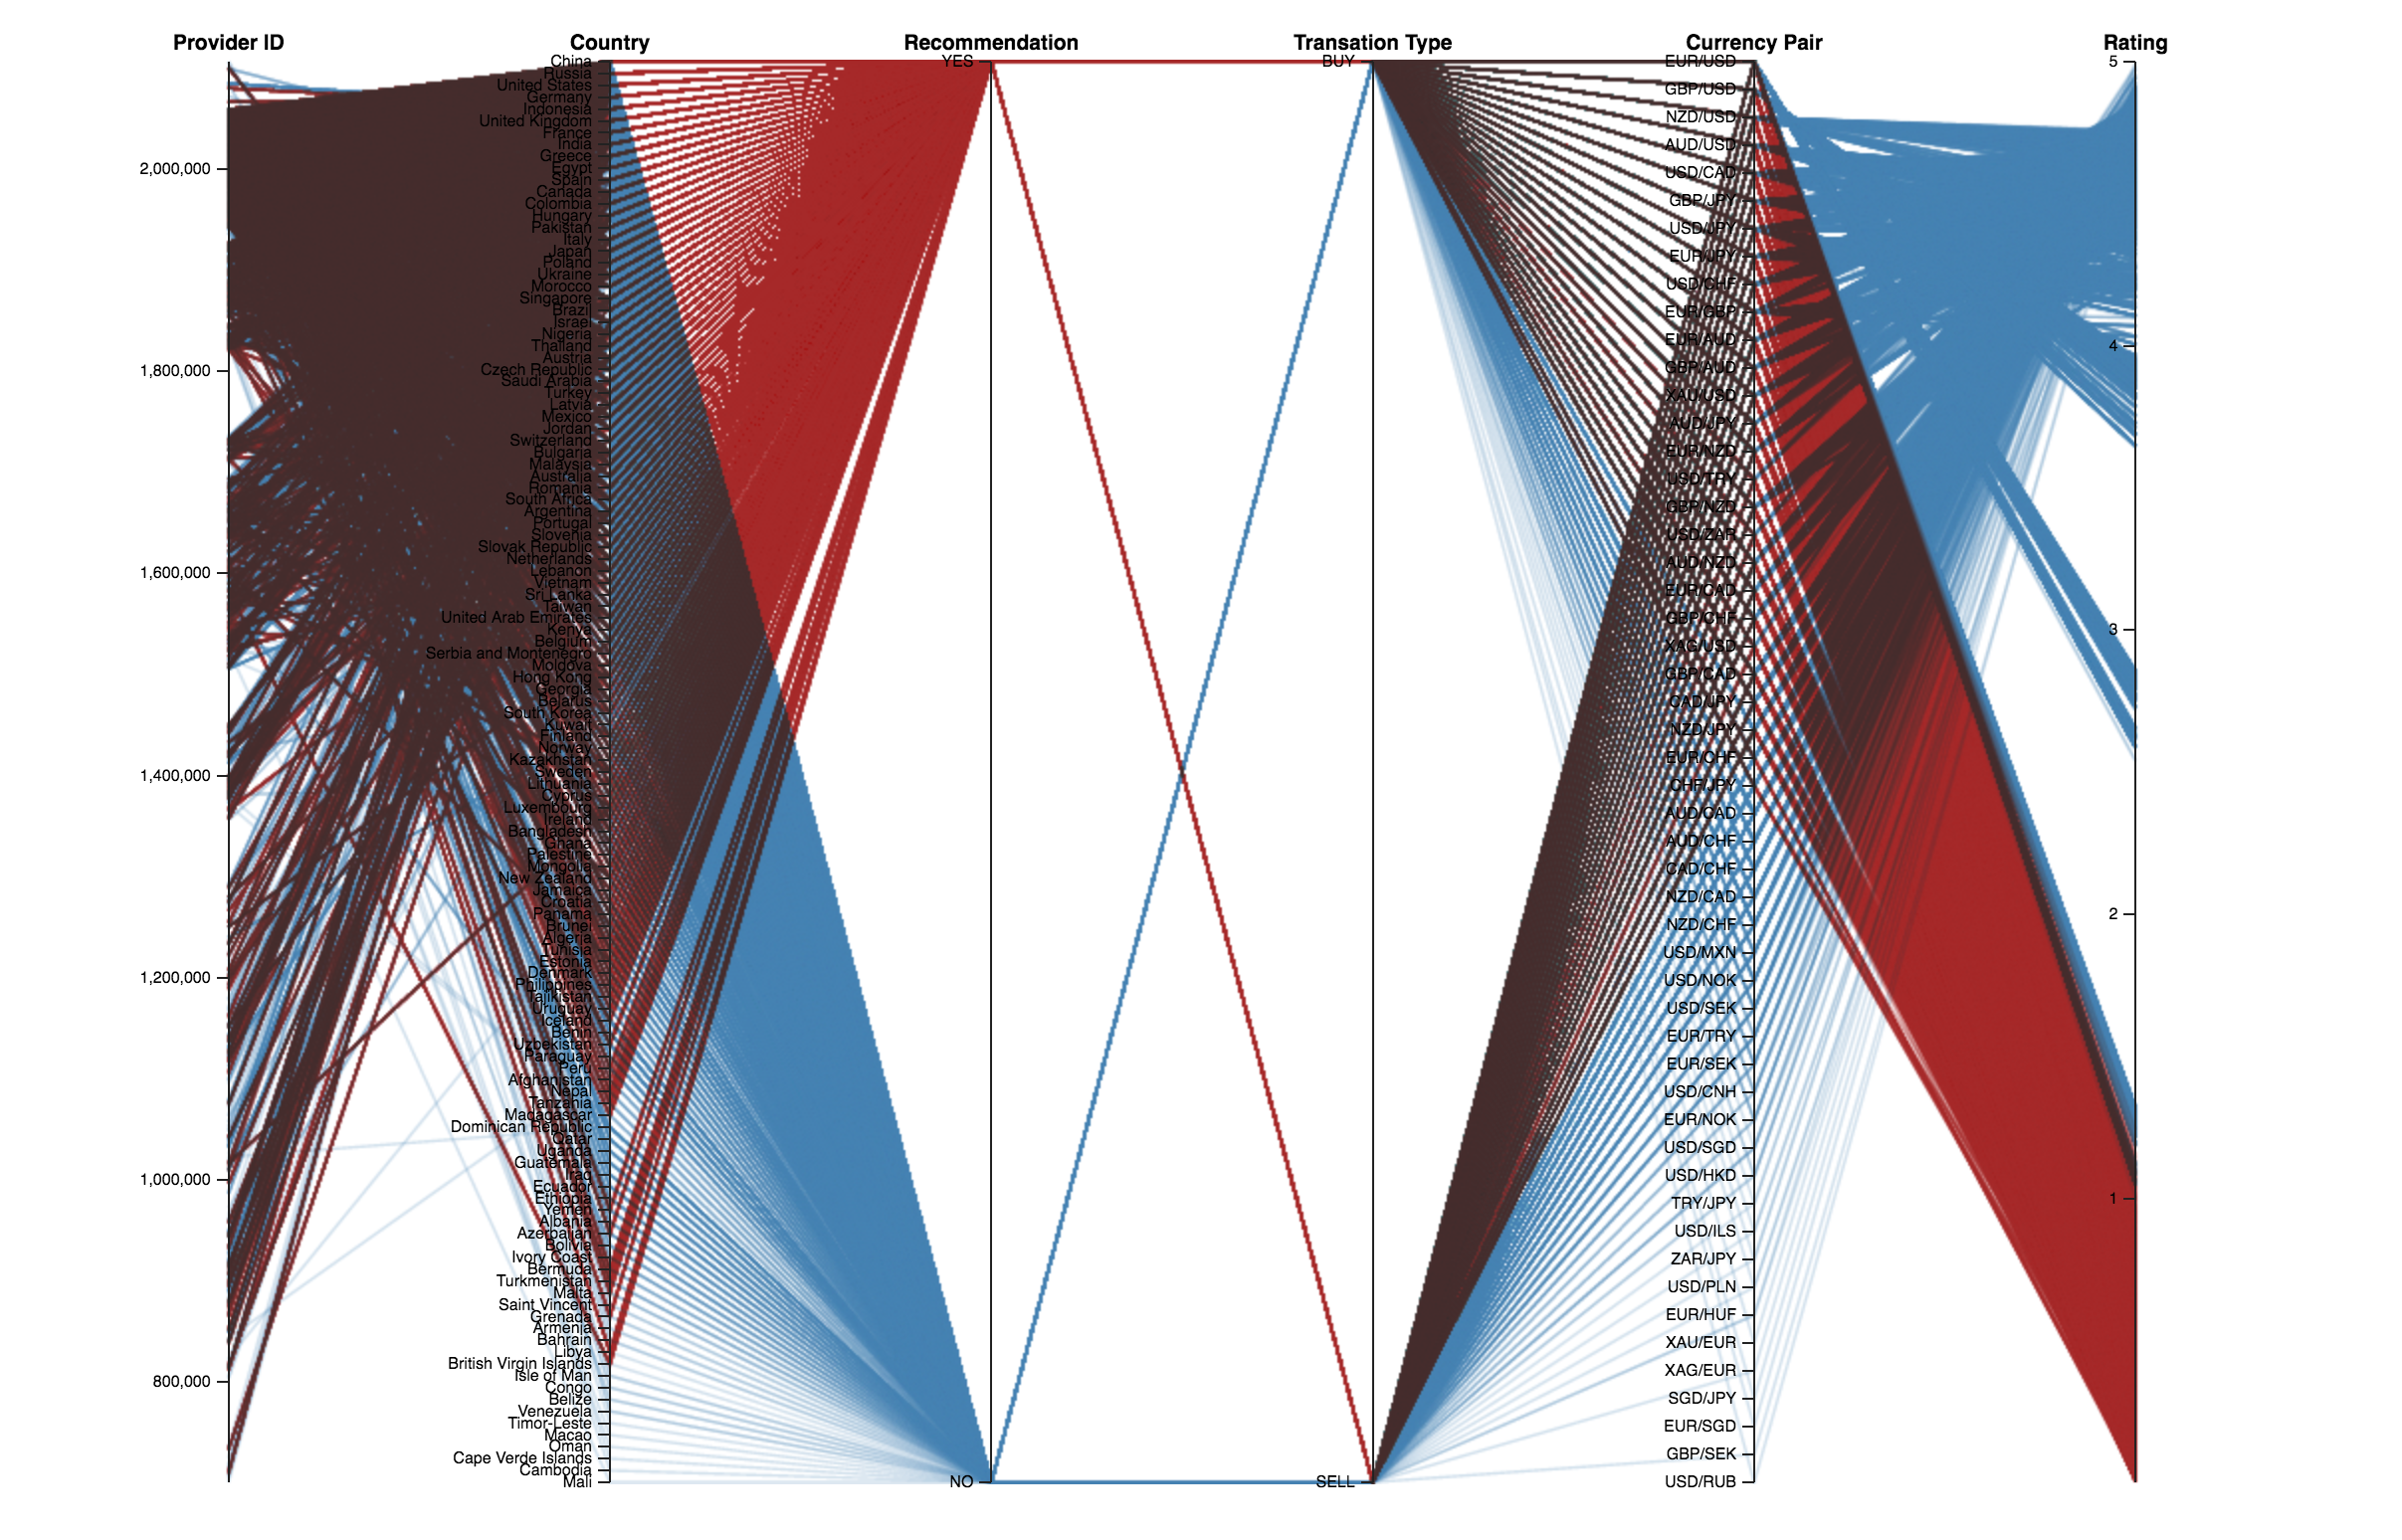
\includegraphics[width=\textwidth]{recommendations_1}
  \label{fig:recommendations_1}
\end{figure}

Στη συνέχεια μπορούμε να επιλέξουμε συγκεκριμένους χρηματιστές και να δούμε τις συναλλαγές που πραγματοποίησαν στο διάστημα το οποίο είχαμε χρησιμοποιήσει για να εκπαιδεύσουμε το RS, τις συναλλαγές που τους προτείναμε για την επόμενη μέρα, αλλά και τι όντως έπραξαν την επόμενη μέρα, ώστε να αξιολογήσουμε την απόδοση του RS.

\begin{figure}[H]
  \centering
  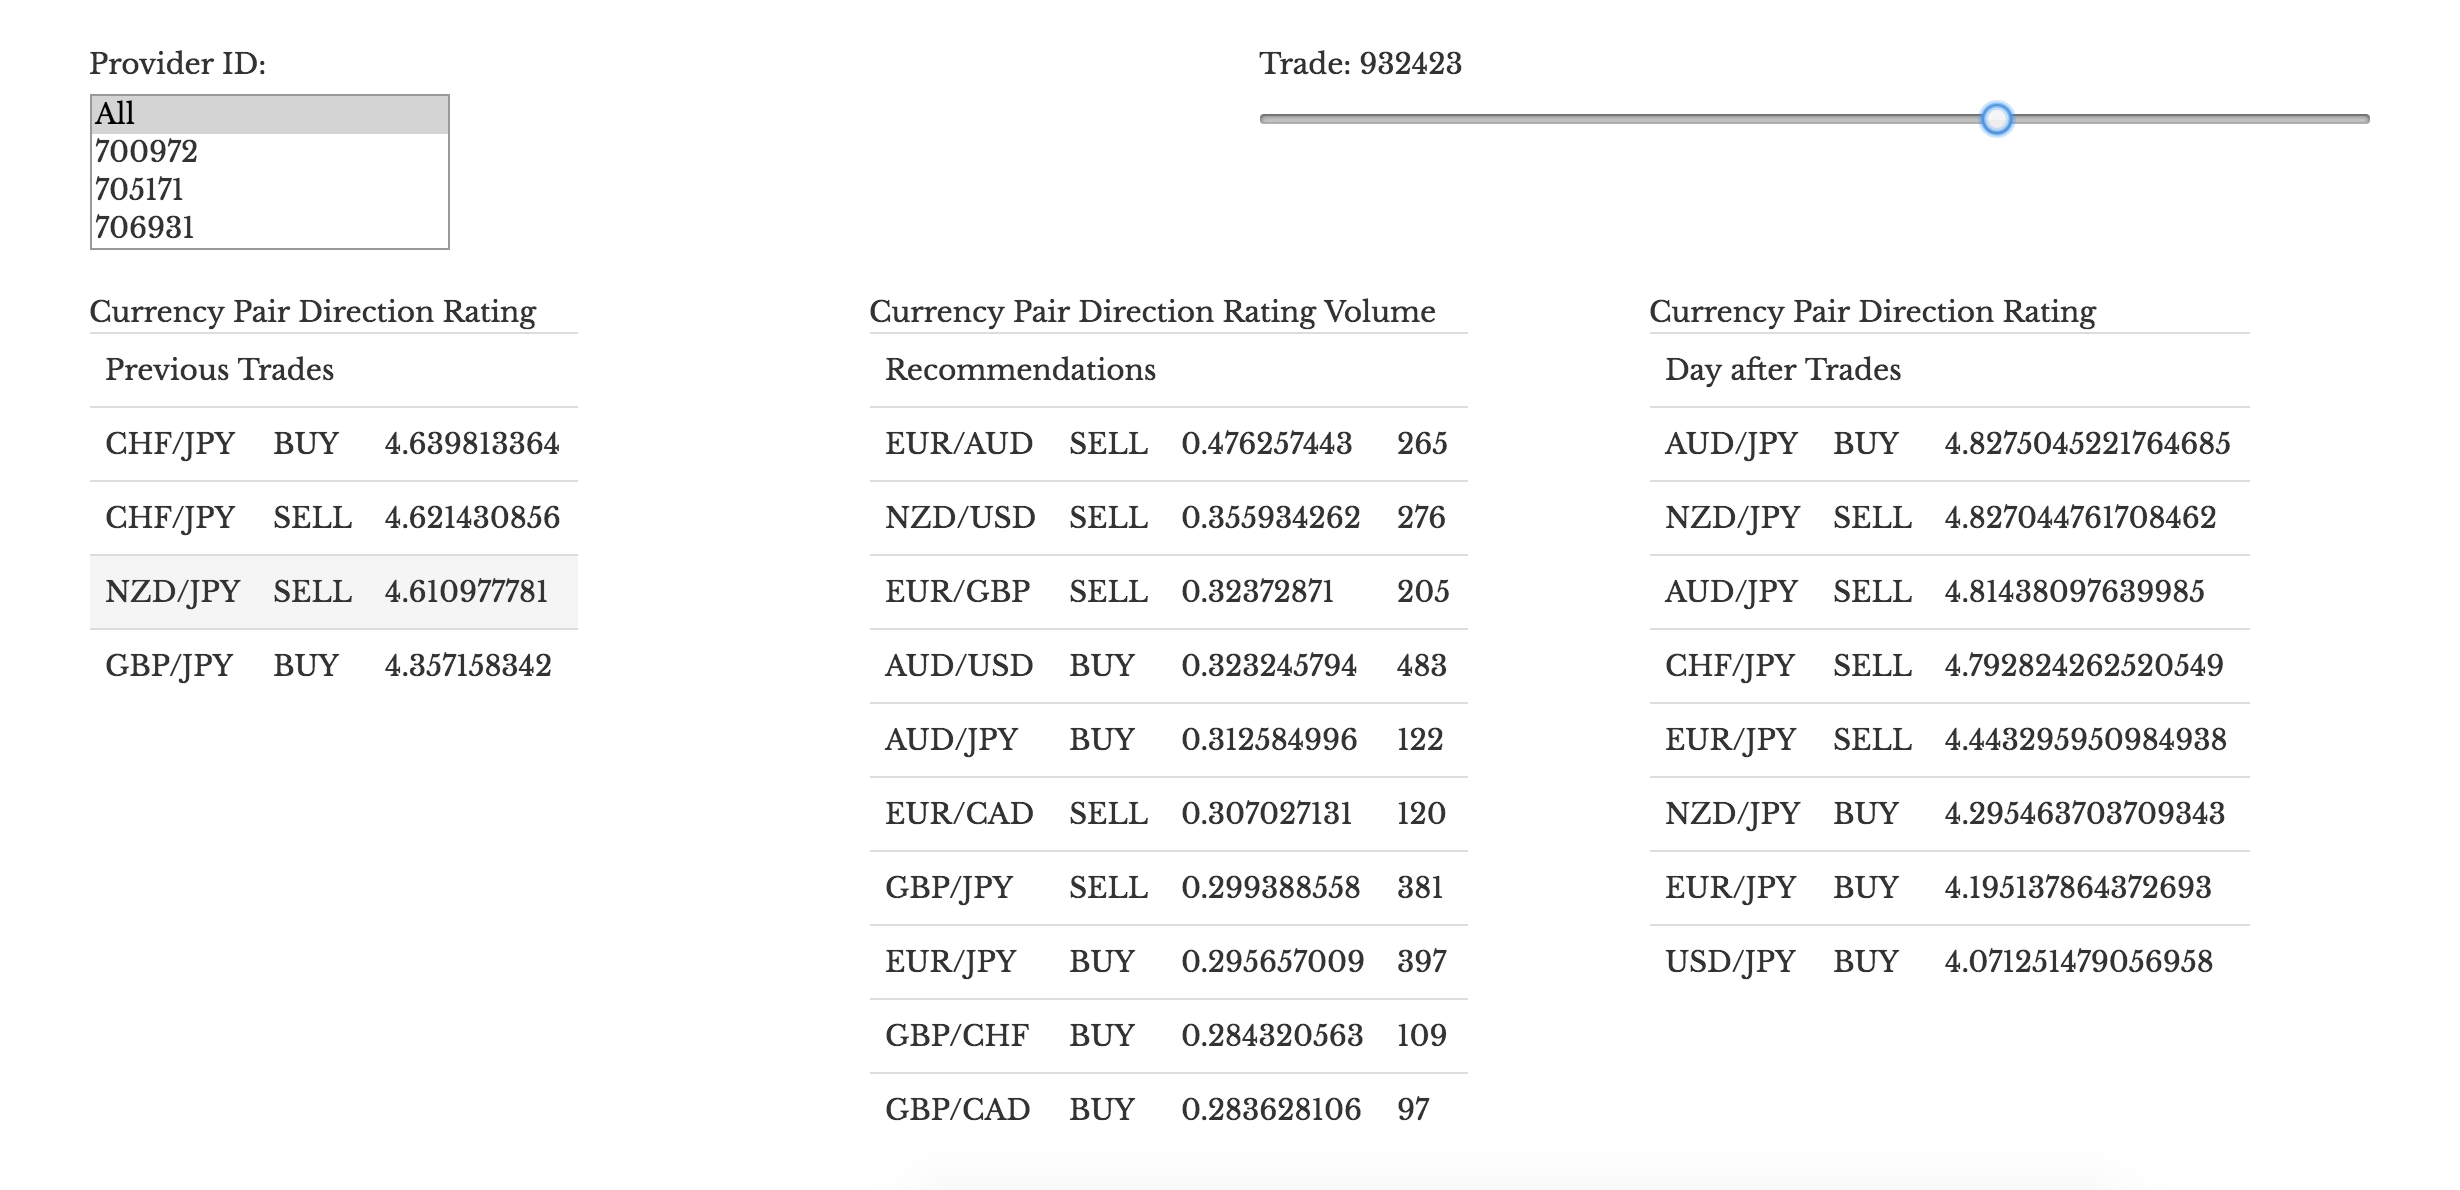
\includegraphics[width=\textwidth]{recommendations_2}
  \label{fig:recommendations_2}
\end{figure}

\begin{figure}[H]
  \centering
  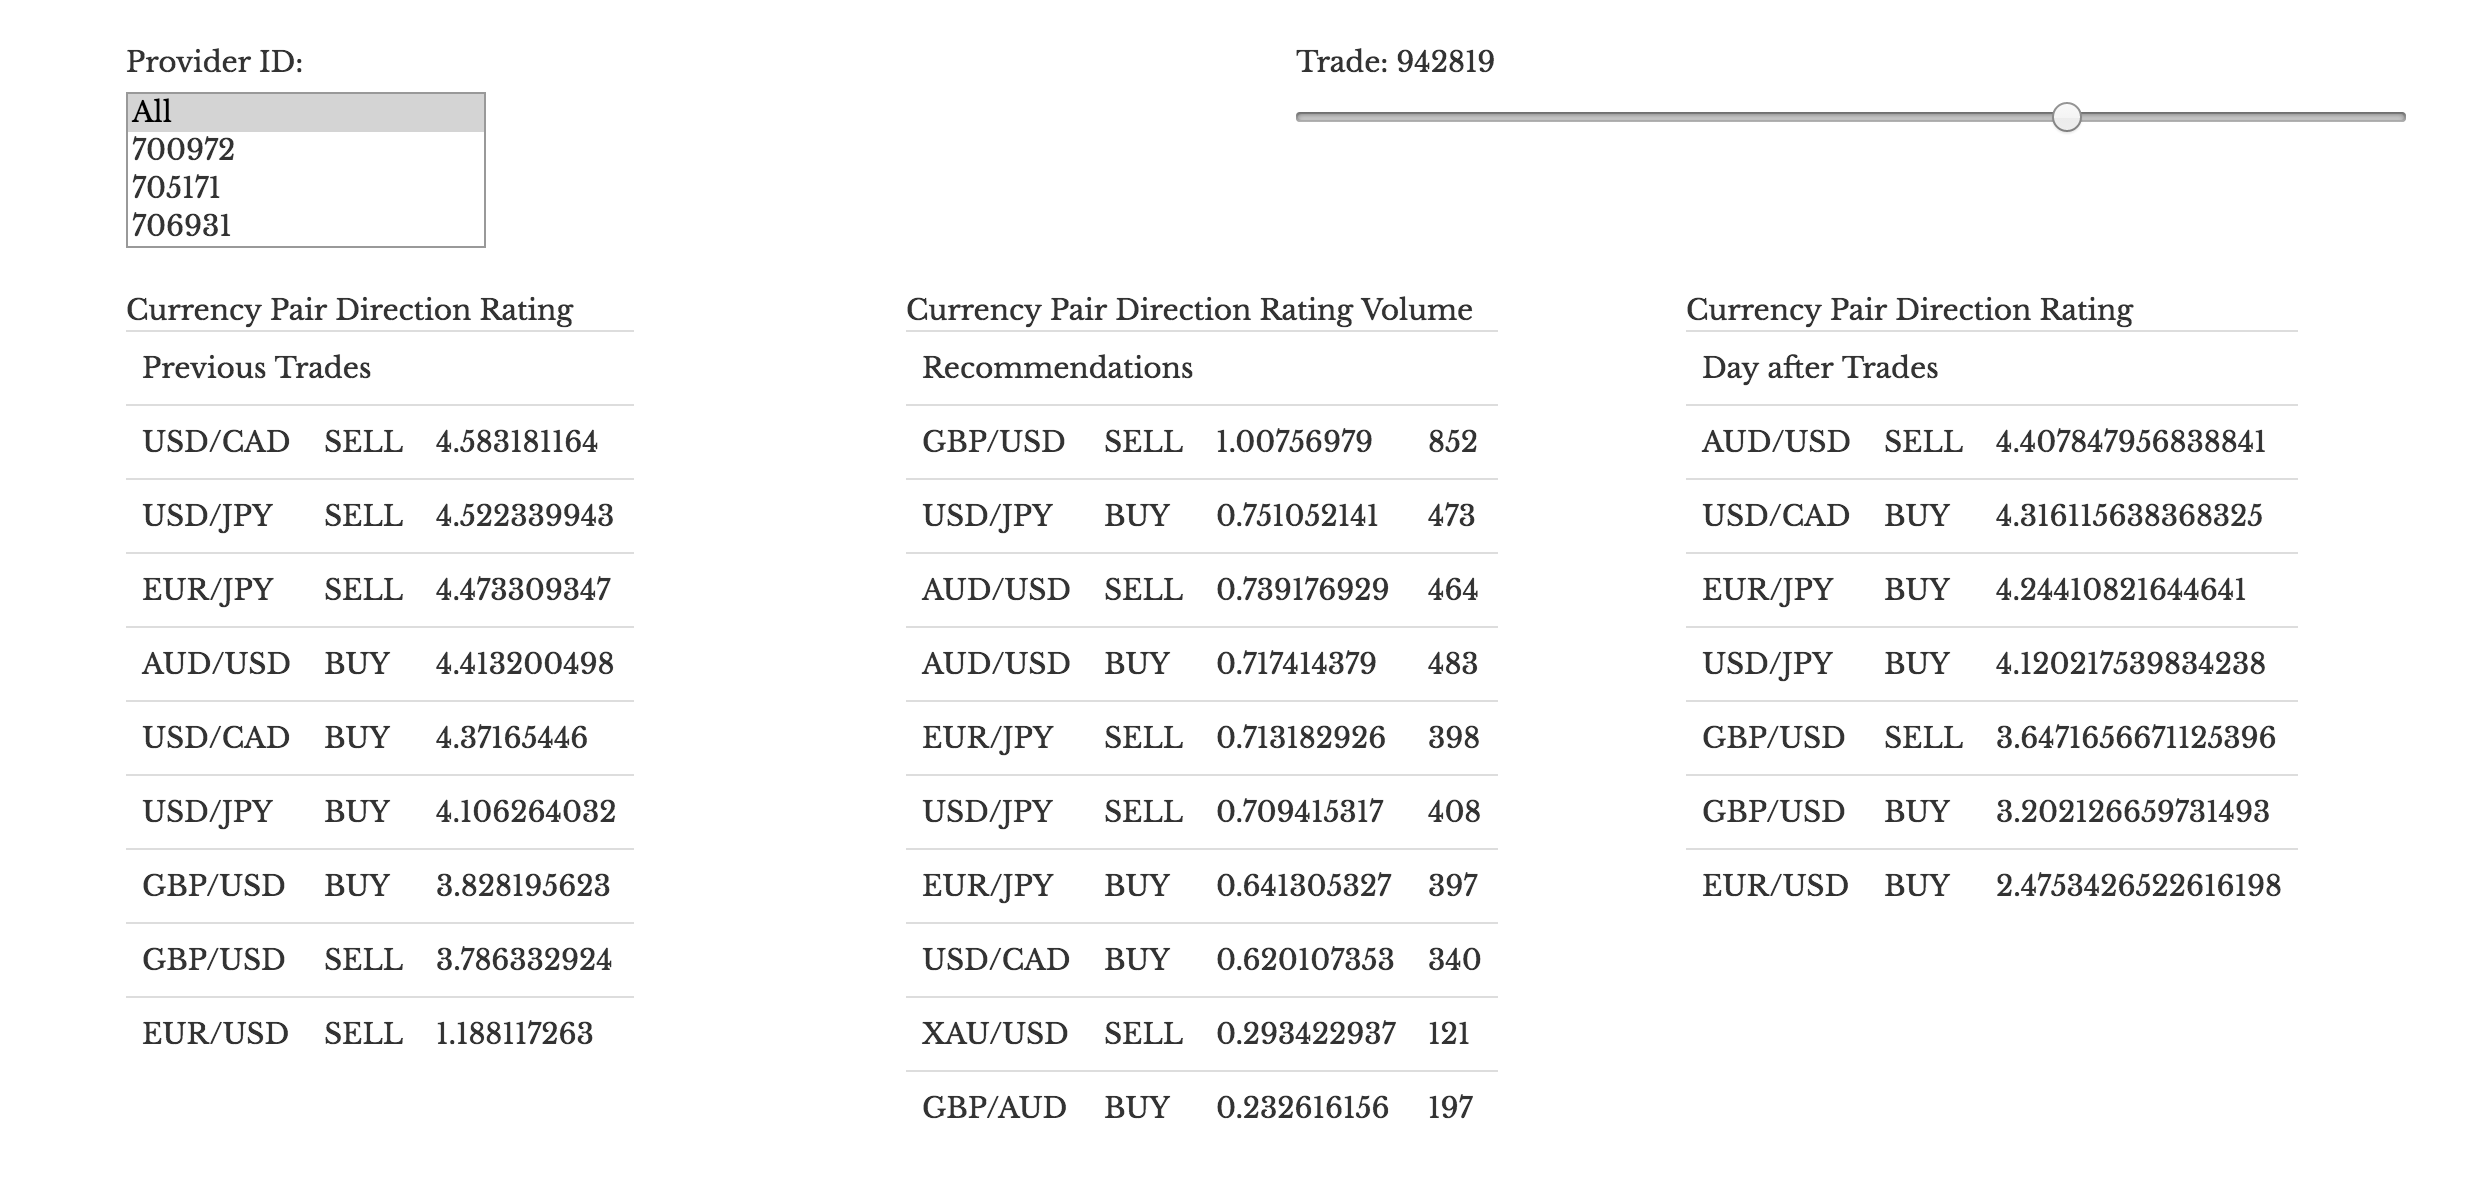
\includegraphics[width=\textwidth]{recommendations_3}
  \label{fig:recommendations_3}
\end{figure}

Όπως βλέπουμε παραπάνω υπάρχει αντιστοιχία στις περισσότερες περιπτώσεις μεταξύ των συστάσεων και των συναλλαγών που πραγματοποίησε ο χρηματιστής την επόμενη εβδομάδα. Αυτό που παρατηρείται σε πολλές περιπτώσεις είναι ότι οι χρηματιστές έχουν ένα σετ από νομισματικά ζεύγη που αγοράζουν ή πουλάνε τακτικά, όμως αυτό δε σημαίνει ότι μία σύσταση πέρα από τα συνηθισμένα ζευγάρια είναι κακή. 

Γι’ αυτό, επίσης παρατίθενται οι τιμές που είχαν πάρει τα νομισματικά ζεύγη που προτείναμε κατά την περίοδο εκπαίδευσης του RS αλλά και τις μέρες που αφορά η παραγόμενη σύσταση ώστε να δούμε αν οι προτάσεις μας θα μπορούσαν να είναι κερδοφόρες σ’ αυτήν την περίοδο, ώστε να αξιολογήσουμε πόσο επικερδής θα ήταν μία συναλλαγή που θα άνοιγε και έκλεινε αυτή την περίοδο. 

\begin{figure}[H]
  \centering
  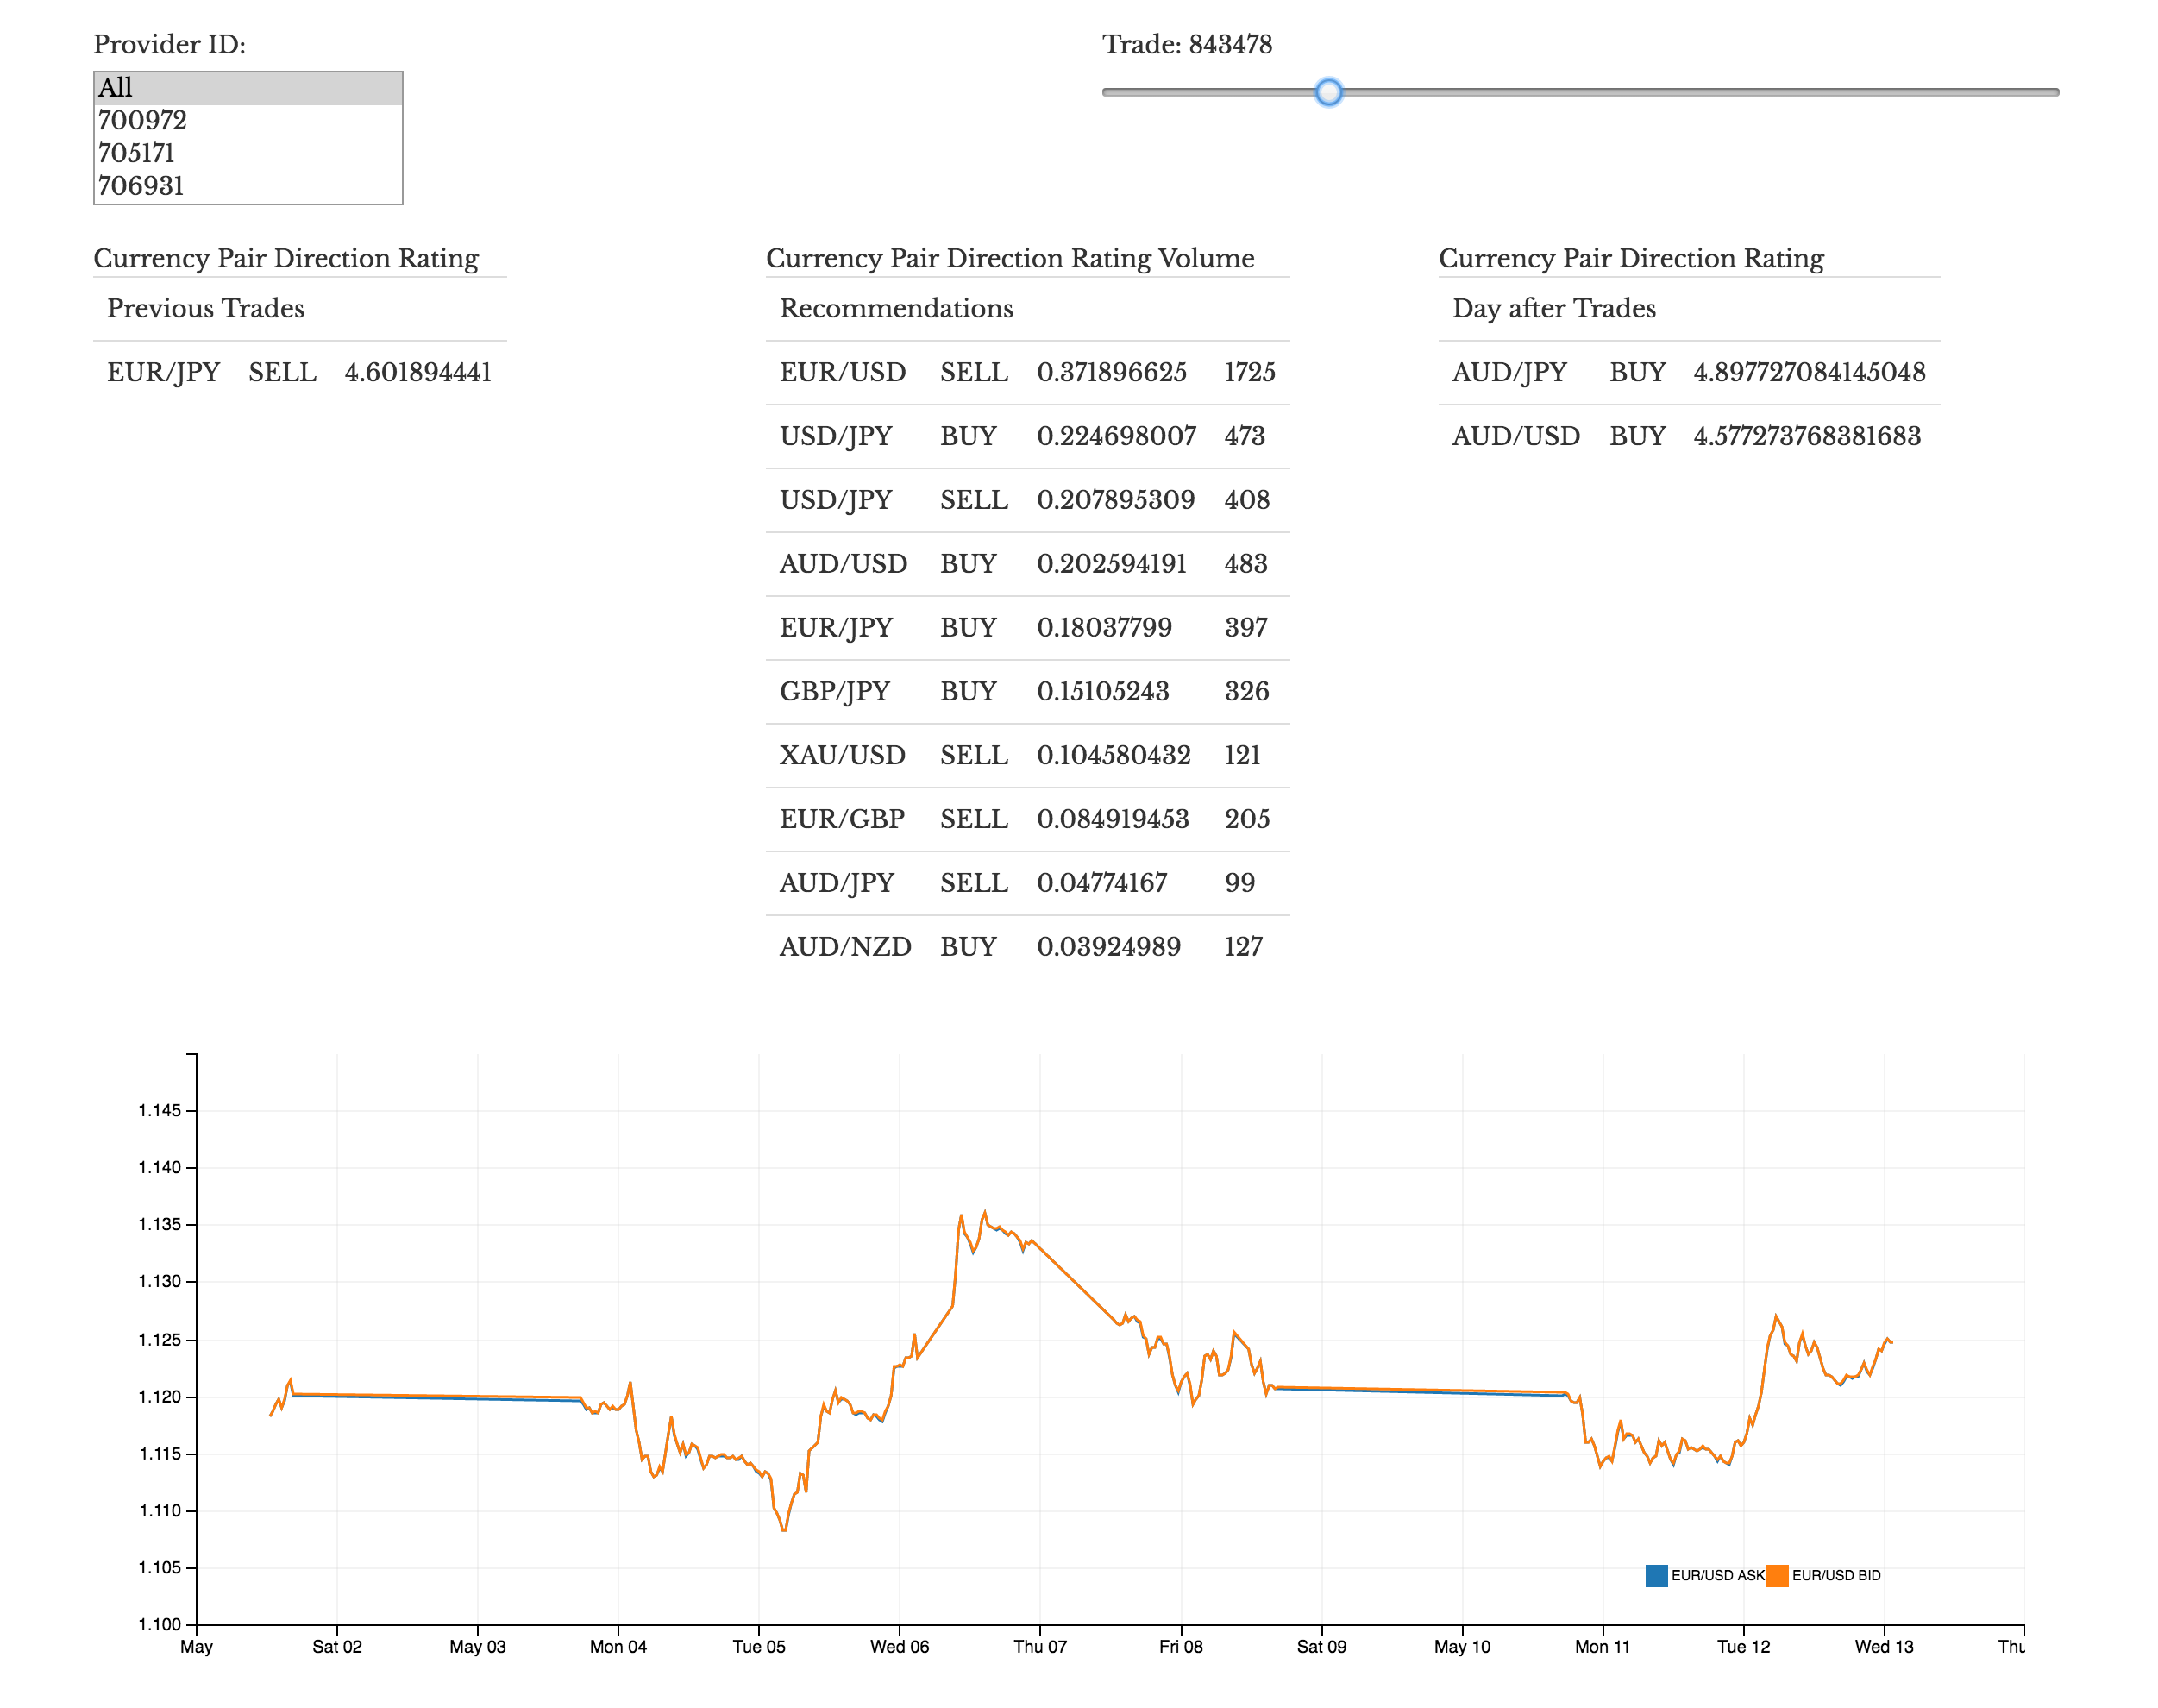
\includegraphics[width=\textwidth]{recommendations_4}
  \label{fig:recommendations_4}
\end{figure}

Όπως βλέπουμε στο παραπάνω γράφημα θα μπορούσε να ανοίξει μία BUY συναλλαγή στο EUR/USD στις 04/05 και να κλείσει στις 07/05 όπου η τιμή αυξήθηκε από 1.118 σε 1.133.

Μ’ αυτόν τον τρόπο μπορούμε να αξιολογήσουμε την ποιότητα του RS συγκρίνοντας τις συστάσεις μας με το τι πραγματικά έκανε ο χρηματιστής, και να δούμε αν χρειάζεται να μεταβάλουμε τα χαρακτηριστικά του RS ώστε να δίνει καλύτερες συστάσεις.

